\documentclass[12pt]{article}
\usepackage{graphicx}
\usepackage{float}
\usepackage{subcaption}
\usepackage{hyperref}
\usepackage{mathtools}
\usepackage[usenames,dvipsnames]{xcolor}
\usepackage[authoryear]{natbib}
\usepackage{amsmath}
\usepackage{amsfonts}
\usepackage{bigints}
\usepackage{array}
\usepackage{tikz}
\usepackage{longtable}
\usepackage{geometry}

\bibliographystyle{plainnat}

\setlength{\parskip}{\baselineskip}
\setlength{\parindent}{0pt}

\newcommand{\e}[1]{{\mathbb E}\left[ #1 \right]}
\newcommand{\given}{\mid}
\newcommand{\secref}[1]{``\nameref{#1}''}


\newcommand{\gb}[1]{{\it\color{magenta}{(#1)}}}
\newcommand{\plr}[1]{{\it\color{purple}{(#1)}}}
\newcommand{\gc}[1]{{\it\color{blue}{(#1)}}}

\geometry{a4paper}

\title{Inferring Continuous and Discrete Population Genetic Structure Across Space}
\date{\vspace{-5ex}}
\author{
Gideon S. Bradburd$^{1,a}$, 
Peter L. Ralph$^{2,b}$, 
Graham M. Coop$^{3,c}$}

\begin{document}

\maketitle

\textsuperscript{1}
Department of Integrative Biology, 
Ecology, Evolutionary Biology, and Behavior Graduate Group,
Michigan State University, MI 48824

\textsuperscript{2}
Institute of Ecology and Evolution,
Department of Mathematics,
University of Oregon, Eugene, OR 97403

\textsuperscript{3}
Center for Population Biology,
Department of Evolution and Ecology, 
University of California, Davis, CA 95616

\textsuperscript{a}bradburd@msu.edu; 
\textsuperscript{b}plr@uoregon.edu;
\textsuperscript{c}gmcoop@ucdavis.edu\\\\\

\newpage
 

\begin{abstract}
One of the classic problems in population genetics is the characterization 
of discrete population structure when the genotyped samples also show 
continuous patterns of genetic differentiation.
Especially when sampling is discontinuous, 
clustering or assignment methods may incorrectly ascribe differentiation 
due to continuous processes (e.g., isolation by distance) 
to discrete processes, such as geographic, ecological, or reproductive barriers 
between populations.
This is partly a result of the difficulty of sampling uniformly and continuously 
across the range of a population or species, 
but more, it reflects a shortcoming of current methods for inferring and 
visualizing population structure from genetic data in the face of data 
that are characterized by both continuous and discrete population structure.
Here, we present a novel statistical framework for the simultaneous inference 
of continuous and discrete patterns of population structure.
The method estimates ancestry proportions for each 
sample from a set of discrete population clusters, 
and, within each cluster, estimates a rate at which relatedness decays with distance.
This model explicitly addresses the ``clines vs. clusters" problem in 
modeling population genetic variation by jointly accommodating both 
continuous and discrete patterns of differentiation. 
We demonstrate the utility of this approach using both simulations and an empirical application.
\end{abstract}

%evolutionary history of the genotyped samples has also been shaped by geographically continuous processes, 
%such as migration.


\newpage
\section*{Introduction}
The fundamental goal of evolutionary genetics is to link patterns of genetic variation 
to the processes that have generated and maintained them.
Often, the first step in the analysis of genetic data is to define evolutionary units of analysis
by delineating discrete populations from which individuals or alleles are sampled \citep{wright1949genetical}.
These units are useful for defining a scope of study in research on selection or local adaptation \citep{},
or on identifying either locally adapted alleles (human skin color, ralph \& coop, gartersnakes) or alleles involved in disease (cystic fibrosis).
Delineating populations can also be useful for informing conservation priorities \citep{}.

There have been many methods proposed to characterize populations,
including generating population phylogenies \citep{CavalliSforza1975, treemix},
$k$-means clustering analyses performed on dimensionality-reduction approaches \citep{}, 
such as principal components analysis \citep{menozzi1978synthetic,novembre_interpreting_2008, price2006eigenstrat},
and model-based clustering approaches \citep[e.g.][]{STRUCTURE, falush2003, hubisz2009,ADMIXTURE, FINESTRUCTURE, huelsenbeck2007inference, Corander2003,TESS}, among others.
Here, we will focus on model-based clustering, the most widely used class of approaches.
These methods each perform best under different specific demographic histories of samples being analyzed,
but all can give misleading results when applied to data that show a continuous pattern of isolation by distance \citep{Wright 1938, 1940, Wright1943}.

A pattern of isolation by distance (IBD) arises when migration in a population is spatially limited \citep{Slatkin1985},
and has been modeled in both spatially continuous frameworks \citep{Wright1943,Malecot1948}, 
in which an individual's parents are found within some radius of that individual's location,
and discrete, ``stepping-stone'' frameworks \citep{Kimura1953},
in which migration occurs only between neighboring demes.
Given the generality of the circumstances that generate a pattern of isolation by distance, 
it is unsurprising that IBD is ubiquitous in nature \citep{meirmans2012,Sexton_etal_2014}.

The ubiquity of isolation by distance presents a challenge for models of discrete population structure,
as it is frequently difficult to determine whether observed patterns of genetic variation are 
continuously distributed across a landscape, or instead are partitioned in discrete clusters.
This problem can be compounded if sampling is done unevenly or discretely across a population or species' range,
and has given rise to a debate in the population genetic literature about whether 
individuals are best described as being drawn from continuous clines or discrete clusters 
\citep[e.g.][]{SerrePaabo2004,rosenberg2005clines}.

Existing model-based clustering approaches can only describe continuous patterns of variation using
discrete clusters, 
and so tend to erroneously describe continuously distributed variation with multiple clusters that 
show spatially autocorrelated cluster membership \citep{Frantz2009,Meirmans2012}.
In analyses of empirical datasets, which often are characterized by IBD,
model-based clustering approaches will therefore tend to overestimate the number of discrete clusters present,
with downstream implications for interpretation of results.
For example, conservation resources might be spread too thinly over areas 
that are spuriously assumed to be discrete management units.
In studies of locally adaptive loci, or of the genetics of disease,
discrete populations may be modeled in separately,
reducing the global power to detect the genomic basis of complex phenotypes.

What is desired, then, is a model-based clustering method that incorporates a spatial element.
and specifically one that uses a model of isolation by distance as a biologically sensible null hypothesis 
for the process structuring observed genetic variation.
With an explicit spatial null, discrete population structure need only be invoked when genetic differentiation 
in the data is above and beyond that expected given some estimated background rate at which divergence 
increases with geographic separation.

In this paper, we present a statistical method for simultaneously 
modeling continuous and discrete patterns of population structure.
We model genetic variation in genotyped individuals as 
partitioned within or admixed across a user-specified number of discrete clusters,
within each of which relatedness decays as a parametric function of the distance between samples.
We also implement a cross-validation approach for comparing and selecting models across different numbers of clusters,
and we demonstrate the utility of our approach using both simulated and empirical data.
The implementation of this method, \texttt{conStruct}, is available as an R package at \href{https://github.com/gbradburd/conStruct}{https://github.com/gbradburd/conStruct}.

\section*{Methods}
\paragraph{Data}
The statistical framework of our approach is conceptually similar to \cite{Wasser2004} and \cite{BEDASSLE}, and \cite{spacemix}.
The genetic data modeled consist of allele frequencies $F$ at $L$ unlinked, bi-allelic single nucleotide polymorphisms (SNPs) genotyped across $N$ samples.
The sample frequency at locus $\ell$ in sample $n$, $f_{n,\ell}$, is calculated by first arbitrarily choosing an allele segregating 
at locus $\ell$ to count, 
then dividing the total number of observations of that counted allele by the total number of chromosomes genotyped at that locus
in sample $n$.
We then calculate the sample covariance in allele frequencies, $\widehat{\Omega}$, as

\begin{equation}
\widehat{\Omega} = \frac{1}{L}  FF^T
\label{sample_covariance}
\end{equation}
\gc{SO IS THIS ACTUALLY the calc given the new diagonal?}


\paragraph{Continuous and discrete differentiation}
We wish to describe the observed patterns of genetic variation as a combination of 
discrete population clusters,
within which genetic variation is continuously distributed, 
and between which sampled individuals or populations can be admixed.
Each of these discrete clusters is modeled as a spatial process where
\gc{allele frequencies covary between geographically close locations,
  but  %%changed as we dont model migration or drif
this covariance is allowed to decay with geographic distance. This 
pattern of spatial decay reflects} how migration between neighboring demes acts 
to homogenize allele frequency changes that arise locally due to
drift, \gc{but that migration is less effective at homogenizing
  between geographic distance demes};
%with this interplay between drift and migration 
resulting in a continuous pattern of isolation by distance within each cluster.
Multiple population cluster processes can co-occur in space, 
leading to discrete jumps in allele frequencies across many loci over small geographic distances,
and the genotyped samples can be admixed between different clusters.

\gc{To model the} continuous decay of allele frequency covariance with geographic distance 
within a cluster \gc{we use a flexible powered-exponential function;
  where the} within-cluster covariance between samples $i$ and $j$ is given by:

\begin{equation}
G^{(k)}_{i,j} = \alpha^{(k)}_0 \left( \text{exp} \left( -(\alpha^{(k)}_D D_{i,j}) ^ {\alpha^{(k)}_2}	\right) \right) + \mu^{(k)}
\label{within_cluster_covariance}
\end{equation}

where $G_{i,j}$ is the covariance function between samples $i$ and $j$ within a cluster,
and the superscript $(k)$ denotes that this function is specific to the $k$th cluster.
The quantity $D_{i,j}$ is the observed geographic distance between samples $i$ and $j$,
the \gc{$\alpha^{(k)}$ parameters control the shape of the decay of
  covariance with distance in the cluster},
and $\mu$ is a parameter that describes the \gc{background allele
  frequency   %%amount of shared drift
  covariance within the cluster. If two samples draw 100\% of their
  ancestry from cluster $k$ then, if they are geographically very
  close ($D_{i,j}=0$) they will have allele frequency covariance
  $\alpha^{(k)}_0 +  \mu^{(k)}$ with their covariance decaying to the
  background level $\mu^{(k)}$ within the cluster for large enough geographic distances.}
The shared drift parameter $\mu^{(k)}$ can be interpreted as the branch length connecting 
the $k$th population to the population ancestral to all modeled
clusters \gc{(see XXX)}. 

\gc{Genotyped samples can draw their ancestry from multiple different clusters,
representing these samples being admixed between the clusters.} 
The admixture proportion of the $i$th sample in the $k$th cluster, $w^{(k)}_i$,
gives the probability that an allele in sample $i$ was derived from
cluster $k$ \gc{($\sum_k w^{(k)}_i =1$).}


We can then describe the covariance between samples $i$ and $j$ across all clusters, $\Omega_{i,j}$,
by summing their within-cluster spatial covariances ($G_{i,j}^{(k)}$ in cluster $k$) across all $K$ clusters
and weighting by the product of those samples' admixture proportions in each cluster
\begin{equation}
\Omega_{i,j} = \gamma + \sum\limits_K w^{(k)}_i w^{(k)}_j
G^{(k)}_{i,j} + \delta_{i,j}\eta_i .
\label{cross_cluster_covariance}
\end{equation}

In addition to the admixture-weighted sum of the within-cluster spatial covariances,
this function contains two terms, $\gamma$ and $\delta_{i,j}\eta_i$.
The first, $\gamma$, describes the global covariance between all samples, 
and arises because all samples \gc{have a base-line covariance as they
  share} an ancestral mean allele frequency at each locus.
In the second term, $\delta_{i,j}$ is an indicator variable that takes a value of 1 when $i$ equals $j$ and 0 otherwise. 
and $\eta_i$ gives the variance specific to sample $i$, 
This term on the diagonal of the parametric covariance matrix \gc{captures} processes shaping variance within the sampled deme, 
such as inbreeding \gc{and the sampling process}.

\paragraph{Likelihood and inference}
\gc{We} assume that the allele frequencies \gc{at each locus
  ($\widehat{F}_{\ell}$) are independent among loci and multivariate normally
  distributed across populations}, 
their sample covariance $\widehat{\Omega}$ 
will be Wishart distributed with degrees of freedom equal to $L$, 
the number of loci genotyped.
Linkage disequilibrium (LD) between loci will decrease the effective number of degrees of freedom, 
which we discuss further below.
The likelihood of the sample standardized allele frequency covariance is therefore given by
\begin{equation}
P(\widehat{\Omega} \; | \; \Omega) = \mathcal{W} \left( L\widehat{\Omega} \; | \; \Omega,L\right)
\end{equation}

We estimate the values of the parameters of the model using a Bayesian approach.
Acknowledging the dependence of the parametric covariance matrix $\Omega$ on its constituent parameters
$w,\alpha,\mu,\eta,\gamma$ and on observed quantiy $D$ with the notation $\Omega(w,\alpha,\mu,\eta,\gamma,D)$,
we denote the posterior probability of the parameters as:

\begin{equation}
P\left( w,\alpha,\mu,\eta,\gamma \;	| \; \widehat{\Omega}, L \right) \propto
P\left(\widehat{\Omega} \; | \; \Omega(w,\alpha,\mu,\eta,\gamma,D) \right)
P(w)P(\alpha)P(\mu)P(\eta)P(\gamma)
\end{equation}

The priors, $P(w),P(\alpha),P(\mu),P(\eta),P(\gamma)$, are detailed in the Appendix,
and the constant of proportionality is the normalization constant.
We use a Hamiltonian Monte Carlo sampling algorithm implemented in the statistical language STAN
\citep{stan, NUTS, stan_lib, rstan} to estimate the posterior distribution on the parameters.
We also present an R package \citep{R} called \texttt{conStruct} that functions as a wrapper 
around this inference machinery.

\gc{
\paragraph{Relationship of this model to non-spatial structure models}

A nice feature of our approach is that our model contains a non-spatial assignment model as a special case. 
Setting $\alpha_0^{(k)}$ to zero for all $k$, we obtain a non-spatial model where
each cluster has its own allele frequency at each SNP, and individuals
draw a proportion of their ancestry from each cluster. This model is
strongly conceptually similar to that of STRUCTURE (and related
approaches ADMIXTURE), the only difference being that our likelihood
assumes that allele frequencies are normally distributed around their
expectations, while the standard assignment methods assume that the
error is binomial distributed (see XXXX). Therefore, to compare the fit
of 


}

\gc{ 
\paragraph{Choice of cluster number and cross-validation}


}


\section*{Results}

\subsection*{Simulations}
We first test the method with scenarios generated using the coalescent simulator \texttt{ms} \citep{Hudson2002}.
To generate discrete population structure, we simulate $K$ discrete clusters,
each of which split from a common ancestor at some point in the past, $\tau_{\text{s}}$,
then diverge for some time without migration between them.
To generate continuous differentiation within each cluster,
at time $\tau_{\text{e}}$ we have each of these discrete clusters instantaneously colonize a lattice of demes,
for which we use a stepping stone model with symmetric migration 
to nearest neighbors (eight neighbors, including diagonals).
Finally, at time $\tau_{\text{a}}$ we generate a single dataset that captures both continuous and discrete patterns of population structure 
by collapsing those $K$ discrete lattices into a single grid of demes sampled from the different clusters
or admixed between them (see Fig \ref{sim_setup}).
We simulated datasets under $K =$ 1 through 3, 
sampling 10,000 unlinked loci from each of 20 haploid individuals from every deme
(for details on all simulations, see Methods and Supplementary Materials).

\begin{figure}
	\centering
		{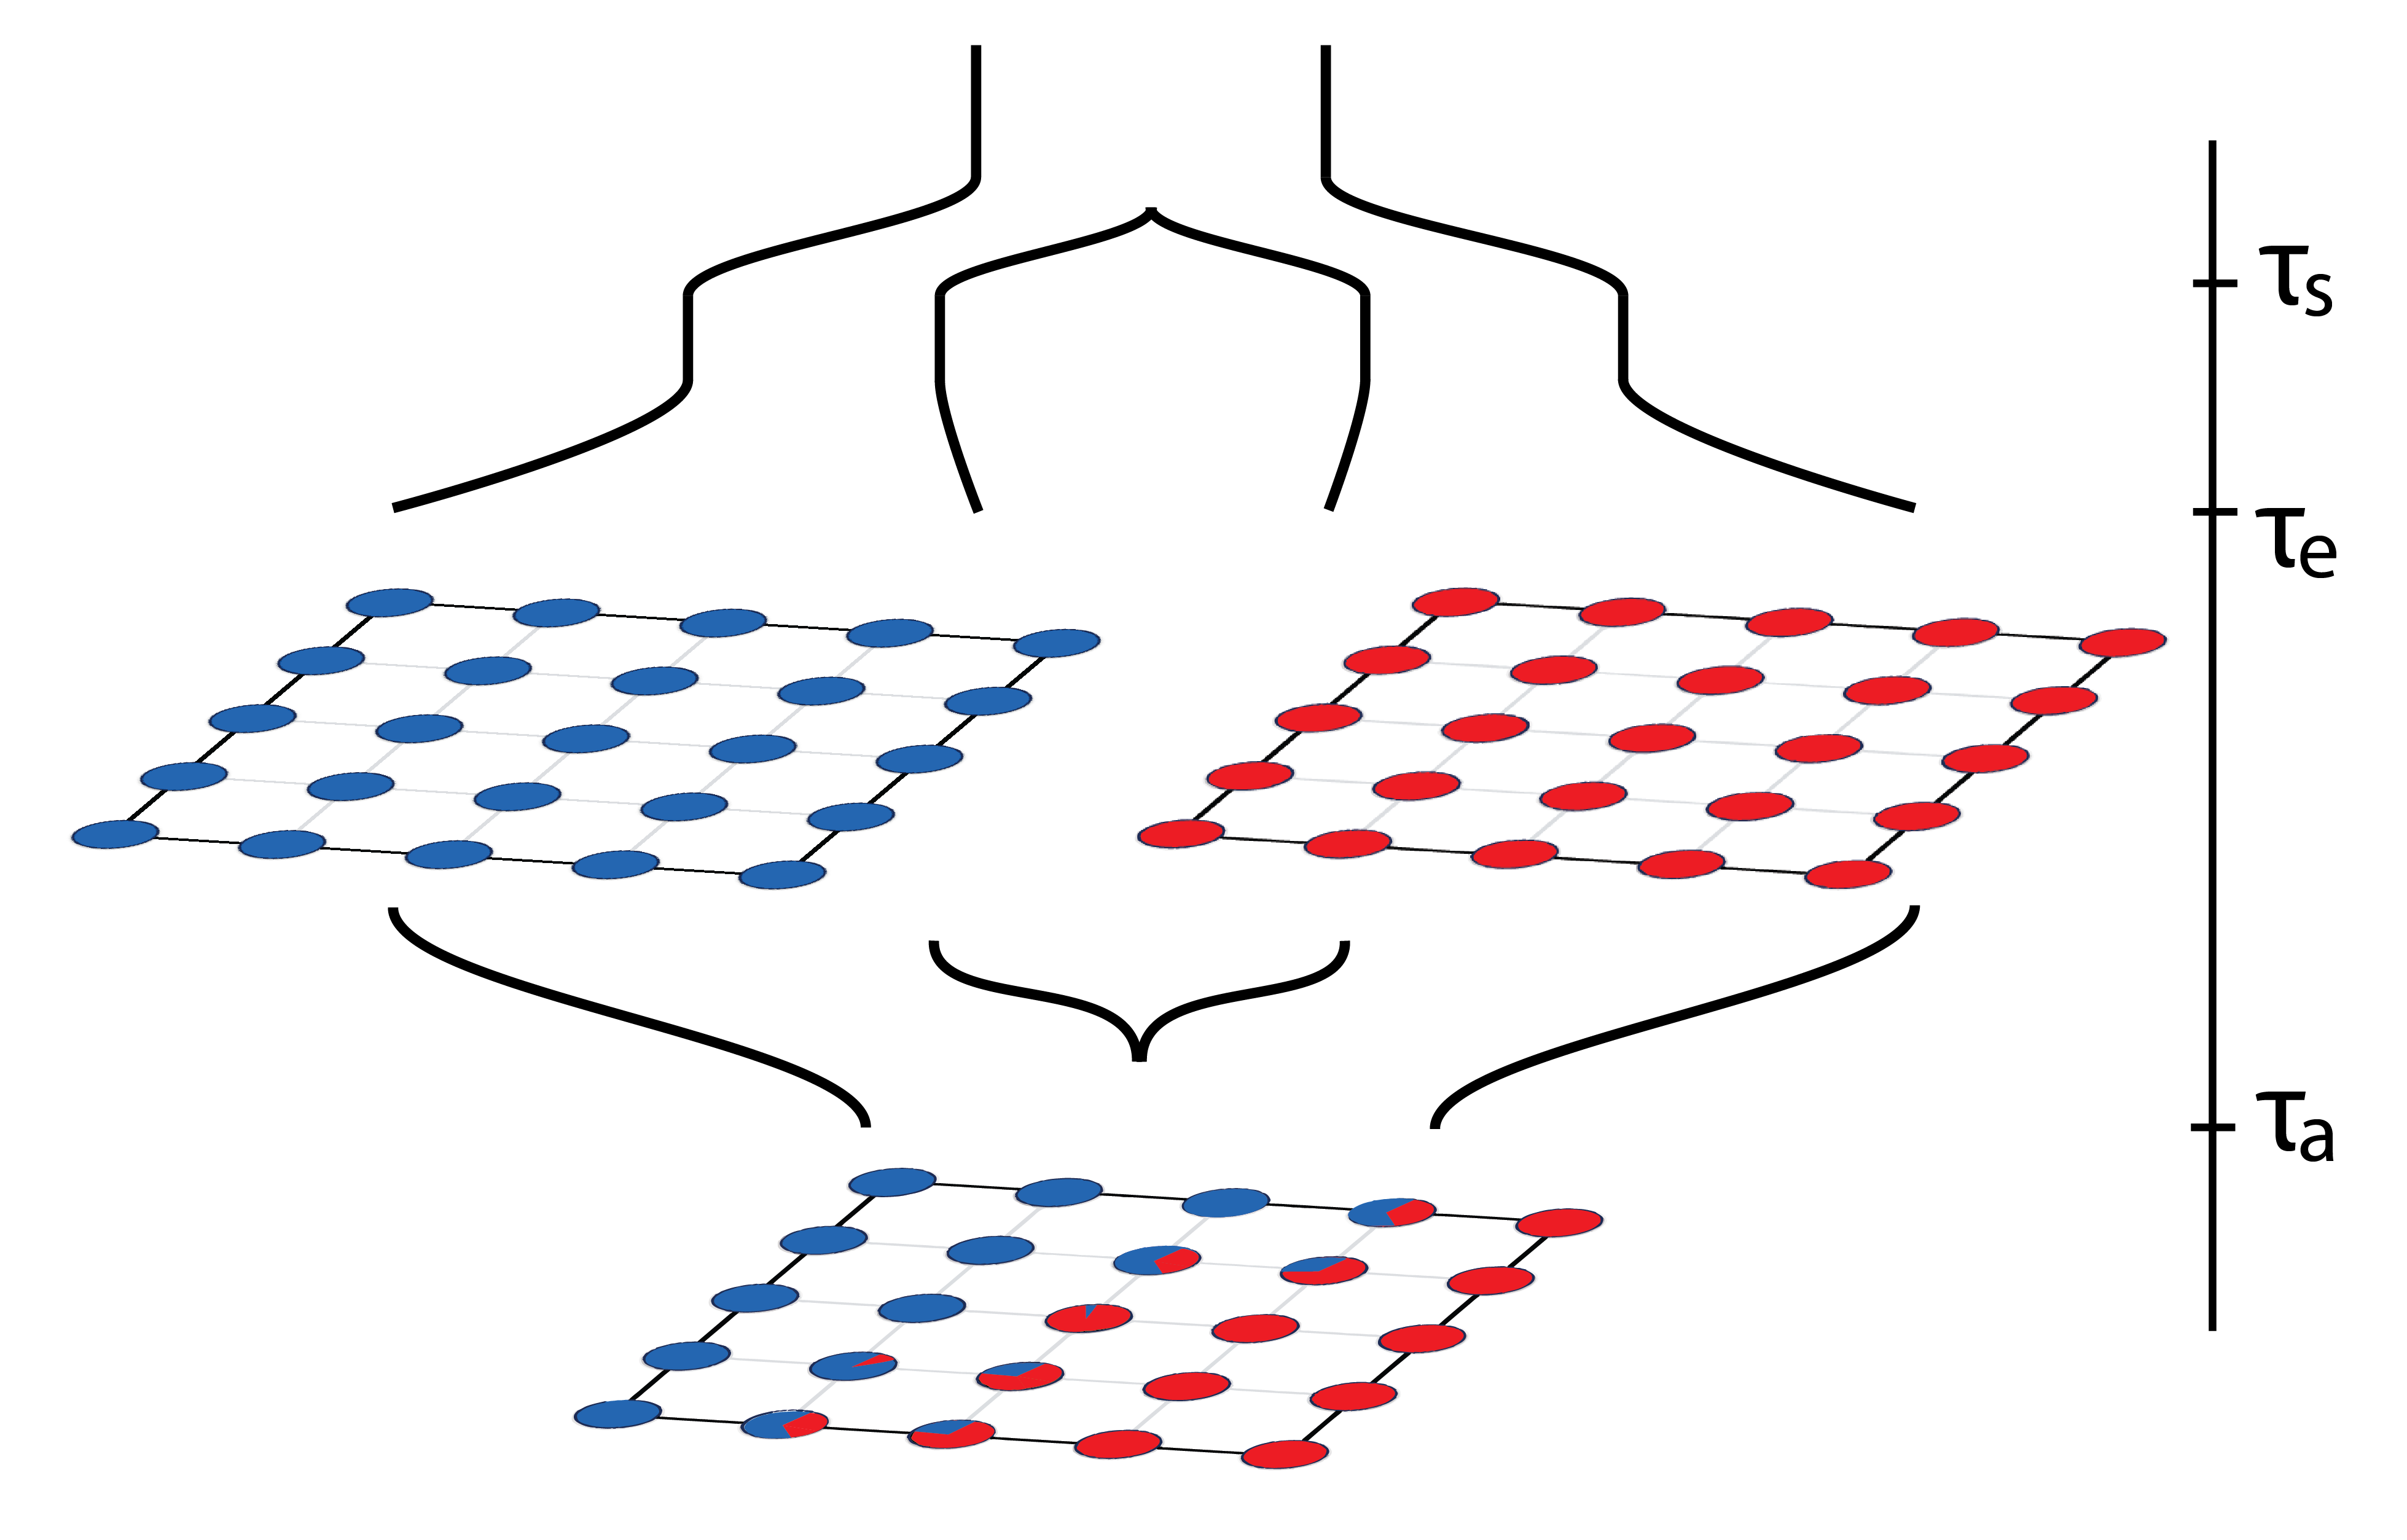
\includegraphics[width=4in,height=2.5in]{figs/sims/sim_setup.png}}
		\caption{Schematic of how we simulate datasets with continuous and discrete differentiation, using $K=2$ as an example.  
			    Going forward in time, the $K$ clusters split from a common ancestor at time $\tau_{\text{s}}$,
			    then each expand to colonize a lattice of demes with nearest-neighbor symmetric migration at time $\tau_{\text{e}}$,
			    then finally at time $\tau_{\text{a}}$ collapse into a single lattice consisting of demes 
			    with ancestry entirely in one or the other of the clusters,
			    or admixed between them.
			    }\label{sim_setup}
\end{figure}

We ran \texttt{conStruct} analyses on each of these simulated datasets, 
specifying both a spatial and nonspatial model for $K = $ 1 through 7, 
then used cross-validation to compare the predictive performance of the models.
In Fig \ref{simK1_nsp_pies}, we show the results of the nonspatial model 
run with between 1 and 7 clusters, applied to the dataset simulated under $K=1$,
and in Fig \ref{xvals} we show the results of the cross-validation analysis for each of the three simulated datasets.
The admixture pie plots for the spatial and nonspatial models run on the datasets simulated under $K=2$ and $K=3$
are shown in Figs \ref{simK1_sp_pies}-\ref{simK3_sp_pies}.

A number of results are immediately clear from these tests with simulated data.
First, across all values of K and for all simulations, 
the spatial model is preferred over the nonspatial model
(this is not surprising, as the data were simulated under a spatial model).
Second, the predictive accuracy of the nonspatial model increases with the number of clusters in the model, 
as it describes continuous, spatial patterns of relatedness between demes within the same cluster 
with gradients of admixture across more and more discrete clusters.
This behavior of the nonspatial model is highlighted in the analyses of data simulated under $K=1$ (Fig \ref{simK1_nsp_pies}):
as $K$ in the model increases, 
the sampled area is increasingly divvied up between clusters 
with ``centers of mass" in the $K$ geographical extremes of the simulated space.
At $K=2$, the clusters are centered in opposite corners on the map; 
at $K=3$, in the lower two corners and the top half; 
at $K=4$, all four corners, and so on.

In contrast, the predictive accuracy of the spatial model of \texttt{conStruct} 
either plateaus at or declines from the true value of $K$ used to simulate the data (Fig \ref{xvals}, second column).
And, as $K$ in the spatial model increases, 
deme membership in clusters beyond the number used to simulate the data does not appreciably increase 
(Fig \ref{simK1_sp_pies}, \ref{simK2_sp_pies}, \ref{simK3_sp_pies}).
That is, even when the spatial model is run with $K=7$, 
the inferred admixture proportions are nearly identical to 
those estimated under the true value of $K$ for each simulation.

\subsection*{Empirical Applications}





\begin{figure}
	\centering
		\subcaptionbox{$K=2$\label{simK1_nsp_pies:K2}}
			{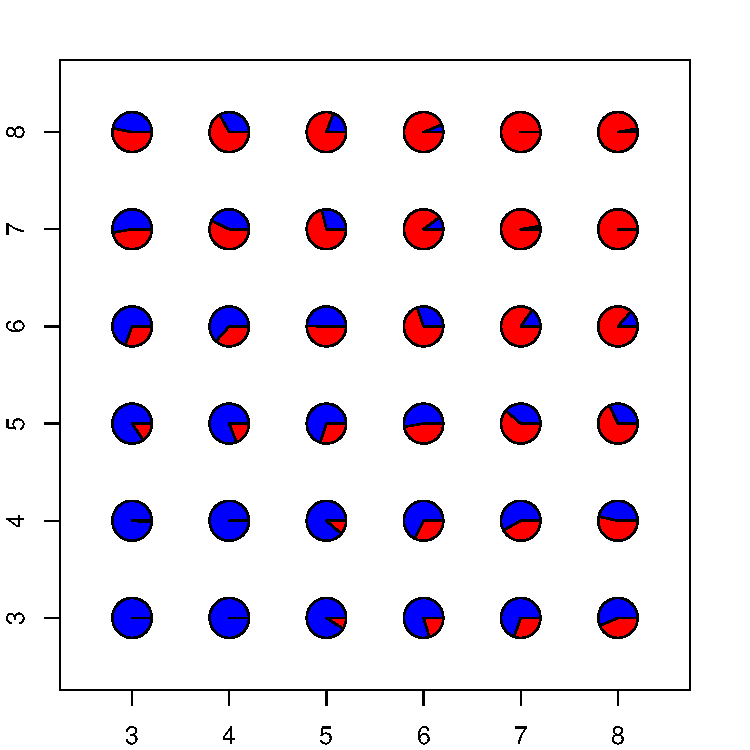
\includegraphics[width=1.8in,height=1.8in]{figs/sims/simK1_nsp_pies_K2.pdf}}
		\subcaptionbox{$K=3$\label{simK1_nsp_pies:K3}}
			{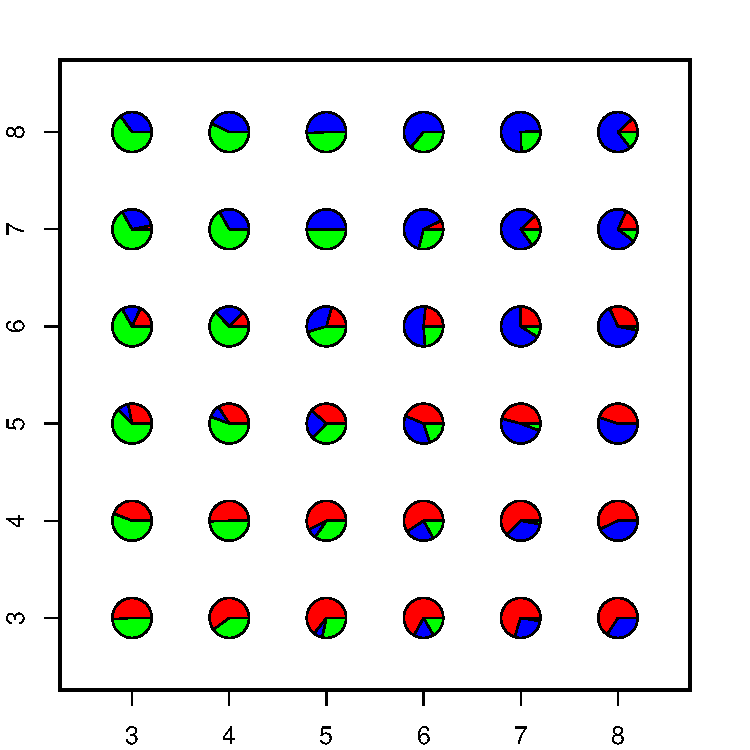
\includegraphics[width=1.8in,height=1.8in]{figs/sims/simK1_nsp_pies_K3.pdf}}
		\subcaptionbox{$K=4$\label{simK1_nsp_pies:K4}}
			{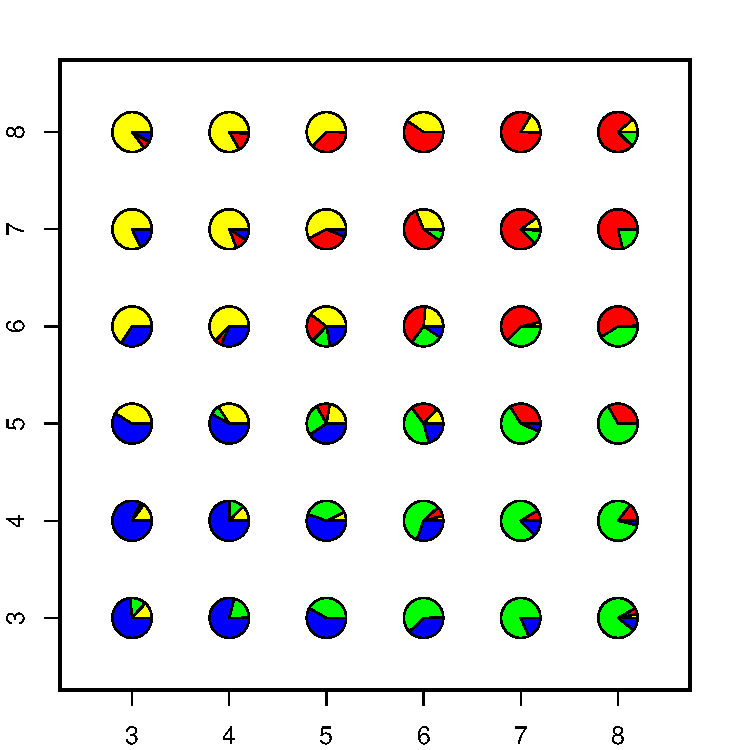
\includegraphics[width=1.8in,height=1.8in]{figs/sims/simK1_nsp_pies_K4.pdf}}
		\subcaptionbox{$K=5$\label{simK1_nsp_pies:K5}}
			{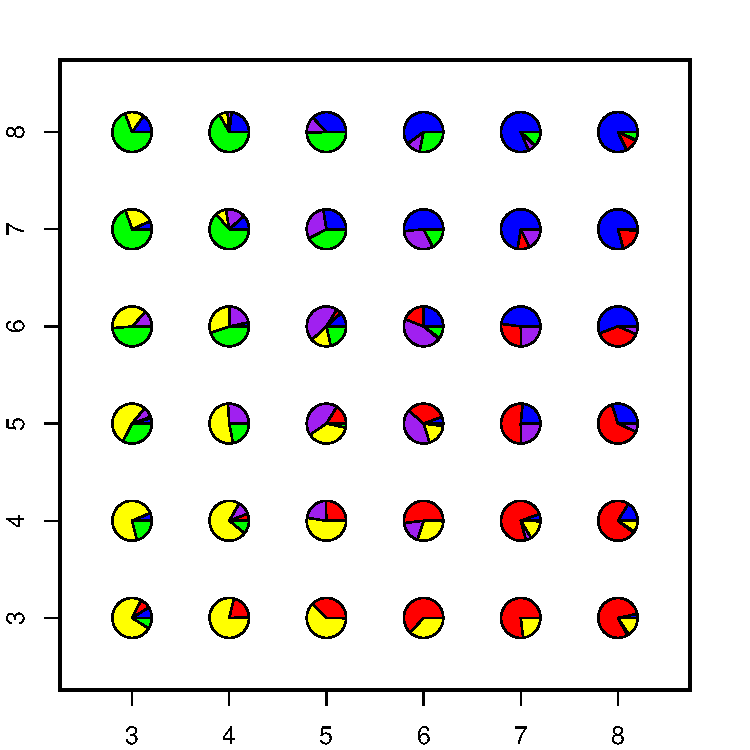
\includegraphics[width=1.8in,height=1.8in]{figs/sims/simK1_nsp_pies_K5.pdf}}
		\subcaptionbox{$K=6$\label{simK1_nsp_pies:K6}}
			{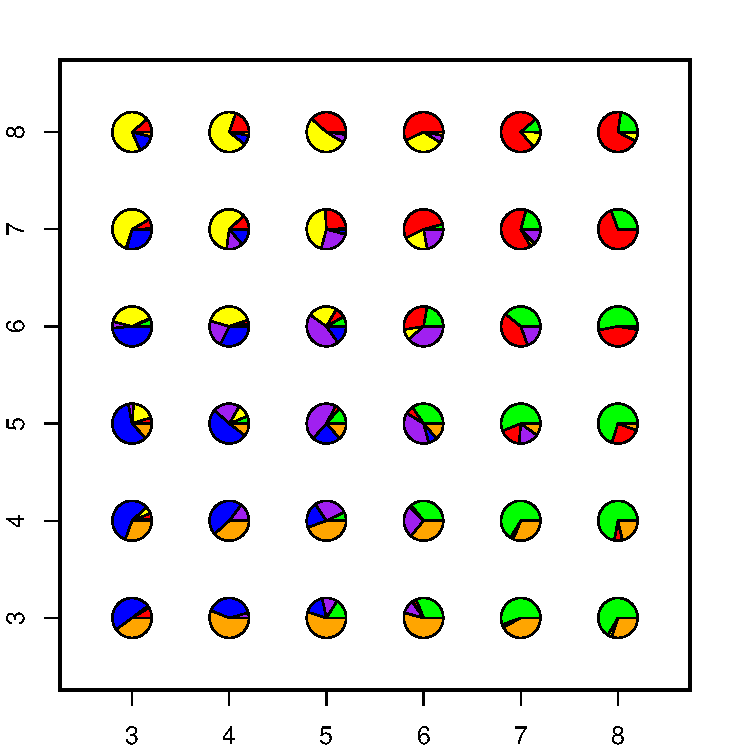
\includegraphics[width=1.8in,height=1.8in]{figs/sims/simK1_nsp_pies_K6.pdf}}
		\subcaptionbox{$K=7$\label{simK1_nsp_pies:K7}}
			{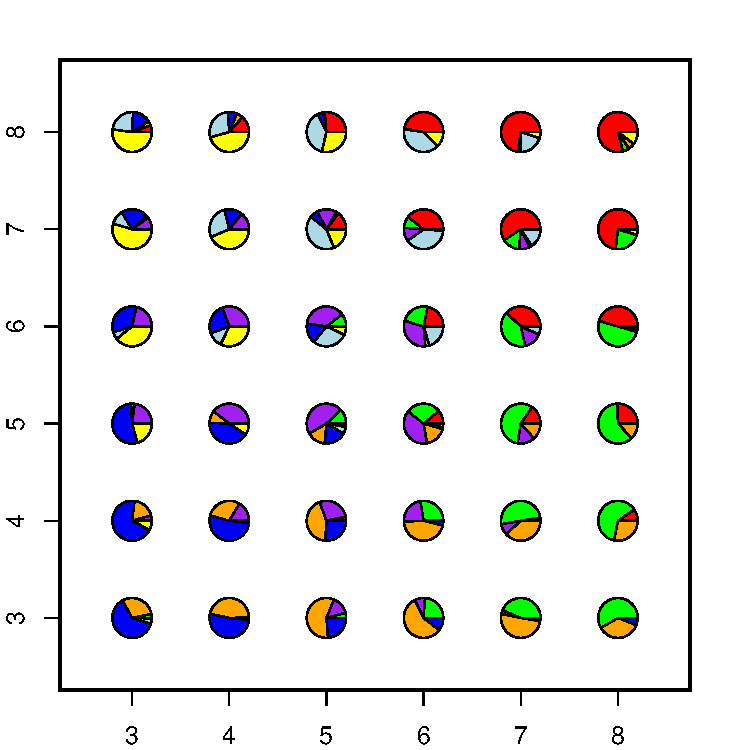
\includegraphics[width=1.8in,height=1.8in]{figs/sims/simK1_nsp_pies_K7.pdf}}
	\caption{
	Map of admixture proportions estimated using a nonspatial model for $K=2$ through 7.
	The data were simulated using a single cluster with nearest-neighbor symmetric migration between demes.
    }\label{simK1_nsp_pies}
\end{figure}

\begin{figure}
	\centering
		{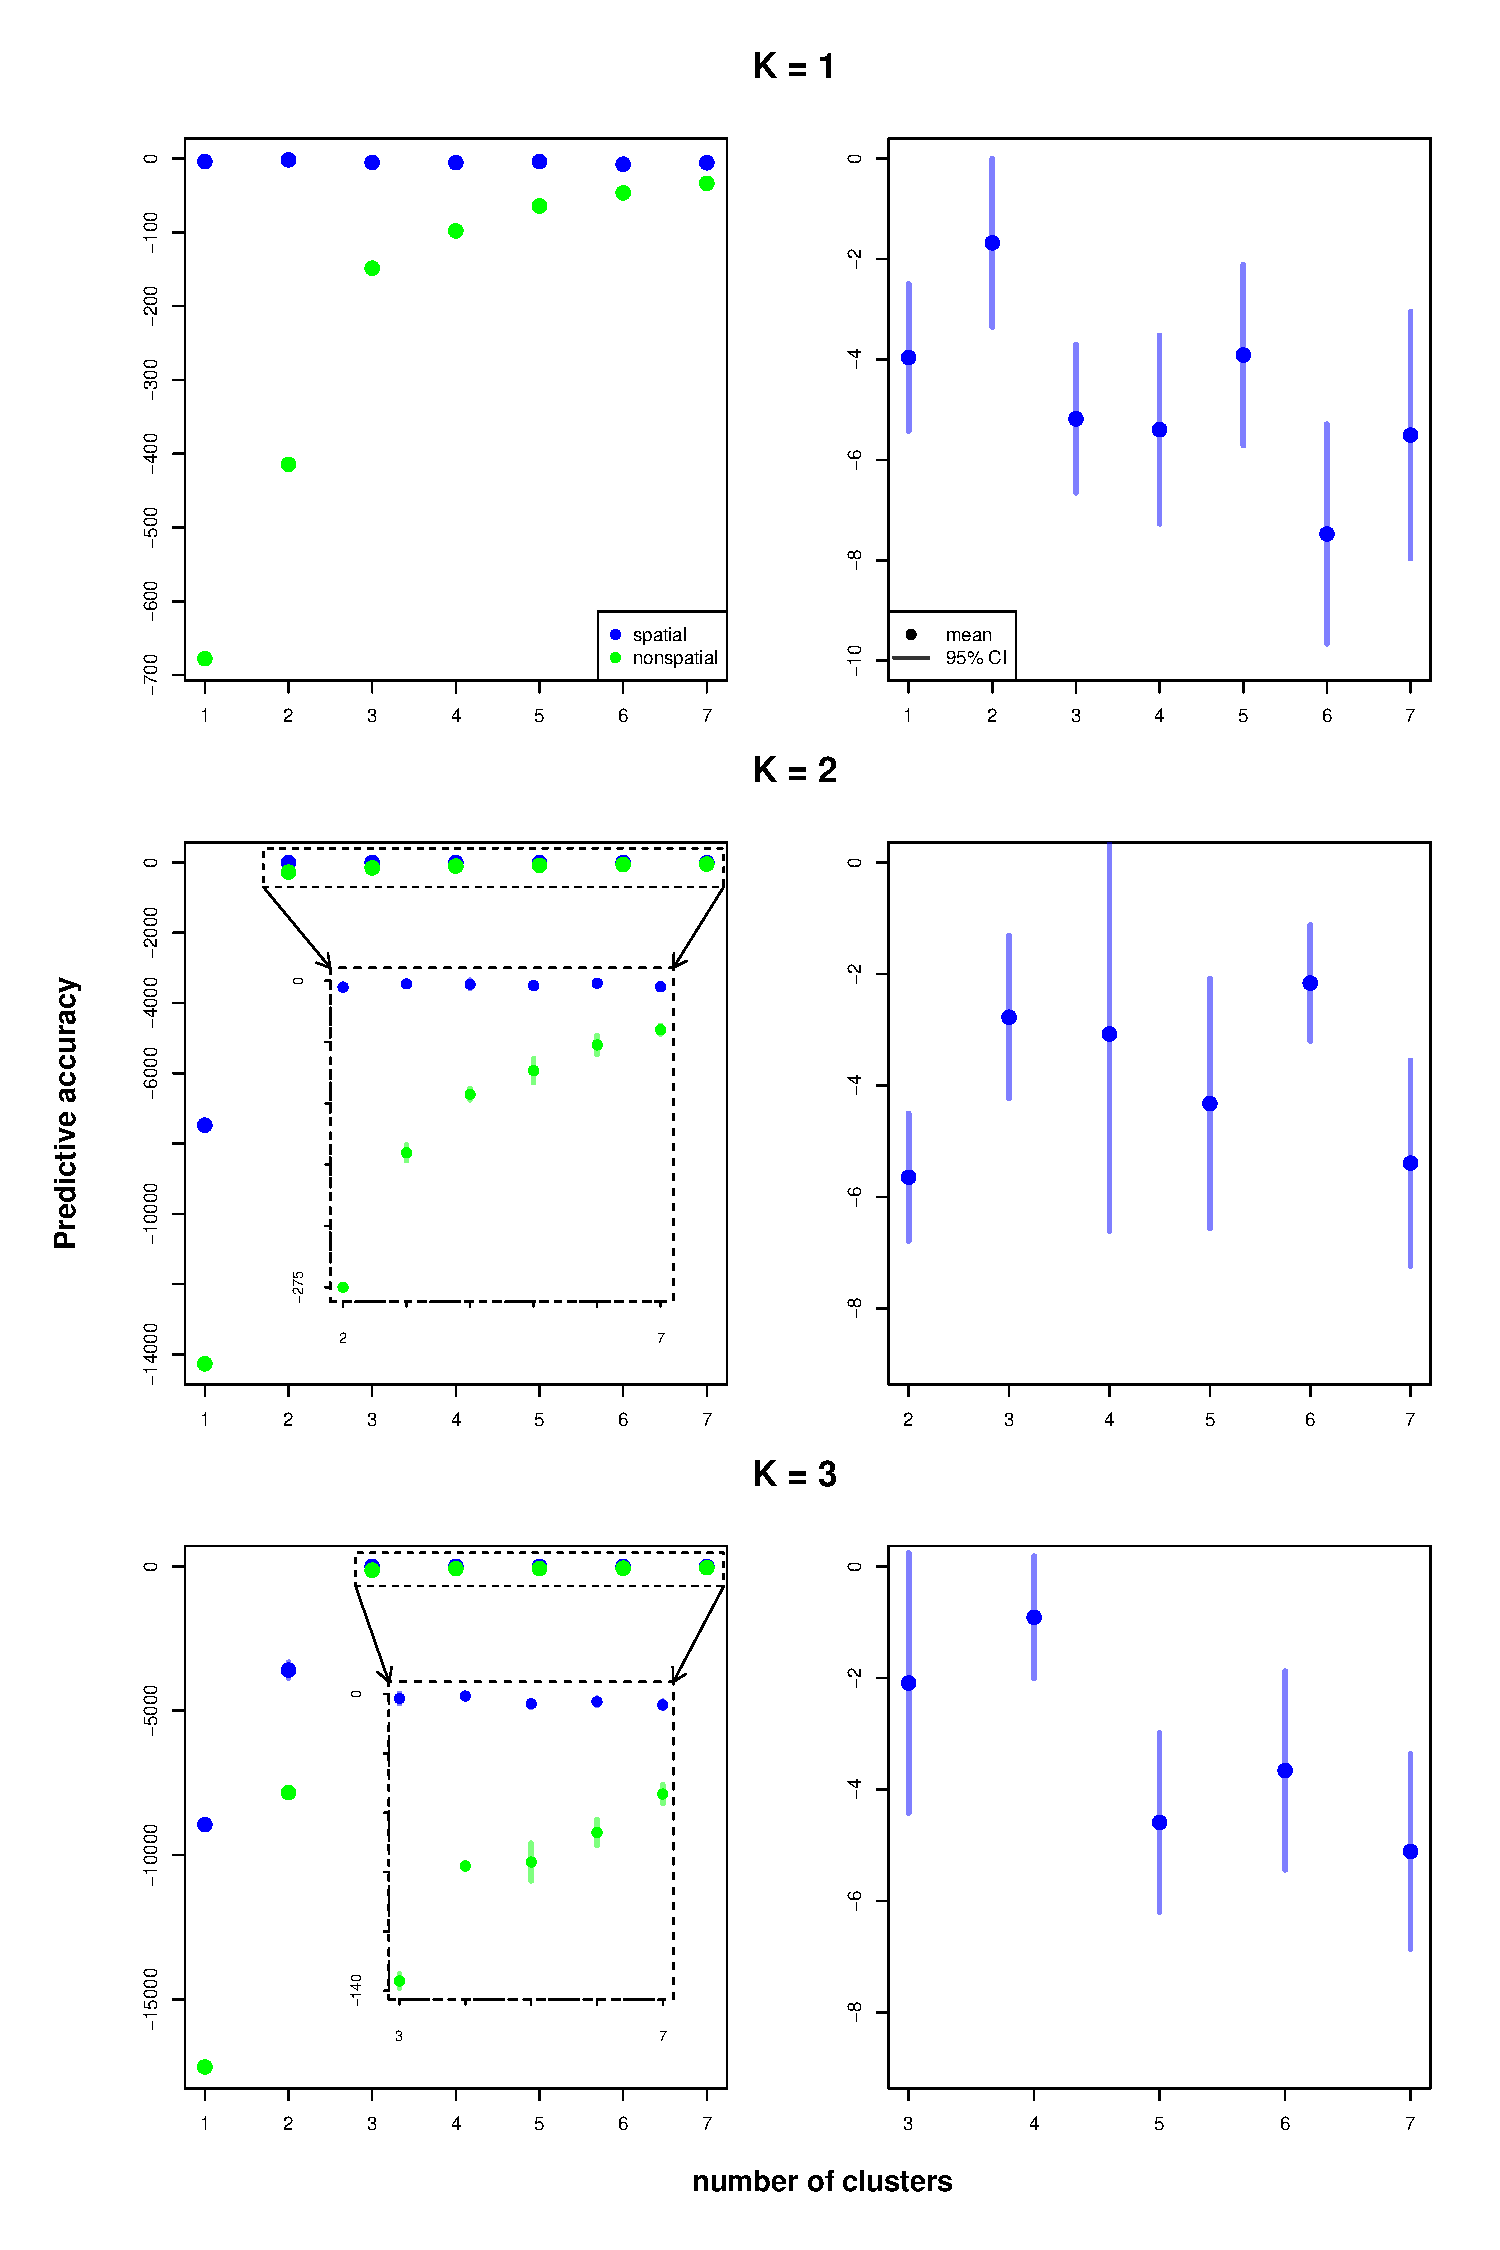
\includegraphics[width=6in,height=8.5in]{figs/sims/xvals.pdf}}
	\caption{
	Cross-validation results for data simulated under $K=1$, $K=2$, and $K=3$, 
	comparing the spatial and nonspatial \texttt{conStruct} models run with $K=1$ through 7.  
	The first panel in each row shows all results; 
	the second panel shows results for just the spatial model.
	The inset plots zoom in on cross-validation results outlined in the dotted boxes.
    }\label{xvals}
\end{figure}


\section*{Discussion}

\section*{Acknowledgements}

We thank Marjorie Weber, William Wetzel, Mariah Meek, Yaniv Brandvain, and Matthew Stephens 
for invaluable comments on the method and manuscript, 
as well as Quentin Cronk, who helped interpret the \textit{Populus} analyses, 
and the attendees at the 2017 SSE Meeting in Portland, OR, whose votes determined the name of the method.
This work was supported in part by 
the National Science Foundation under award number NSF \#1262645 (DBI) to PR and GC, 
the National Institute of General Medical Sciences of the National Institutes of Health under award numbers NIH RO1GM83098 and RO1GM107374 to GC,
and the National Science Foundation under award numbers NSF \# 1148897 and \# 1402725 to GB.

\newpage
\section*{Appendix}
\renewcommand{\theequation}{A\arabic{equation}}
\setcounter{equation}{0}
\renewcommand{\thetable}{A\arabic{table}}
\setcounter{table}{0}
\renewcommand{\thefigure}{A\arabic{figure}}
\setcounter{figure}{0}


\section{Model rationale}
\subsection{Drift, admixture, and allele frequencies}
\paragraph{Drift} 
We imagine that the allele frequencies at each locus in each sample are the sum of 3 components: 
the ancestral allele frequency $\epsilon$ shared by all samples,
the deviation from that ancestral mean in the $k$th population, $\Delta^{(k)}$,
which is shared by all samples with 100\% ancestry in that population,
the deviation specific to the $i$th sample, $\Delta^{(i)}$,
which captures drift not shared by all samples at the population level
(i.e., subpopulation-specific drift due to, e.g., inbreeding).

If all samples drew all of their ancestry from any one of the $K$ clusters,
the  allele frequency in the $i$th sample at the $\ell$th locus would be given by:
\begin{equation}
F_{i,\ell} = \epsilon_{\ell} + \Delta^{(k)}_{\ell} + \Delta^{(i)}_{\ell}
\label{drift_terms_no_admix}
\end{equation}

\paragraph{Admixture} 
The model above describes the simple case 
in which samples draw 100\% of their ancestry from only a single cluster each. 
To accommodate admixture between clusters, 
we can model allele frequencies within samples as linear combinations of the population-specific 
drift terms across the clusters from which they draw ancestry.
To do so, we introduce a term $w^{(k)}_{i}$ that describes the admixture proportion of sample $i$ in cluster $k$,
which can be interpreted as the probability that an allele sampled in the $i$th sample came from the $k$th cluster.
The allele frequency in the $i$th sample at the $\ell$th locus can therefore be written as:
%
\begin{equation}
F_{i,\ell} = \epsilon_{\ell} + \sum\limits_{K} \left( w^{(k)}_{i} \Delta^{(k)}_{\ell} \right) + \Delta^{(i)}_{\ell}	
\label{drift_terms_admix}
\end{equation}
%
where
%
\begin{equation}
\sum\limits_{K}w^{(k)}_{i} = 1
\end{equation}

\subsection{The Normal approximation to drift}
Genetic drift is serial binomial sampling, 
but over short timescales, and for intermediate ancestral allele frequencies, 
we can reasonably model the allele frequencies at each locus across populations as multivariate normal.
This will be a good approximation if the amount of elapsed drift in each sample is relatively small,
as would be expected if time since divergence from a common ancestral population is short,
or effective population sizes are large.

Beginning with the simplest case of two clusters ($K=2$),
with all samples drawing 100\% of their ancestry from either one or the other cluster, 
we can model allele frequencies at locus $\ell$ as:
%
\begin{equation}
F_{\ell} \sim MVN\left(\mu = \epsilon_{\ell} + \iota^{(k)}\Delta_{\ell}^{(k)}, \Sigma = \Omega	\right)
\label{MVN_mean}
\end{equation}
%
where $\iota^{(k)}$ is an indicator variable that equals 1 for samples with 100\% membership in cluster $k$
and 0 otherwise.
In Eqn \eqref{MVN_mean}, all entries of the covariance $\Omega$ have value 0 except the diagonals,
which describe sample-specific drift, and have the following value:
%
\begin{equation}
\Omega_{i,i} = \text{Var}\left( \Delta^{(i)} \right)
\label{MVN_mean_diag}
\end{equation}

%

\subsection{Describing relatedness as a covariance}
However, our data can consist of many loci, 
so it may be computationally impractical to model 
the ancestral, cluster, and sample components of each sampled allele frequency.
Instead, we can describe the covariance induced between samples due to the sharing of the components.
All samples share the same ancestral mean at all loci, 
which leads to a global covariance equal to the variance of the ancestral frequencies across loci.
Likewise, samples that are in the same cluster will have a covariance equal to the variance 
of the cluster-specific deviates from the ancestral frequencies across loci.

In Eqn \ref{MVN_mean} above, we described the relatedness between samples
due to the shared ancestral allele frequency and shared population-level drift
via the mean of the multivariate normal.
We can describe this relatedness as a covariance as follows:

\begin{equation}
	\Omega_{i,j} = 
	\begin{cases}
	      \text{Var}(\epsilon) +  \text{Var}\left( \Delta^{(k)} \right) + \text{Var}\left( \Delta^{(i)} \right), & \text{if}\ i=j\ \\
      	      \text{Var}(\epsilon) +  \text{Var}\left( \Delta^{(k)} \right), & \text{if}\ \iota^{(k)}_i = \iota^{(k)}_j\ \text{and}\ i \neq j \\
	      \text{Var}(\epsilon), & \text{otherwise}
	\end{cases}
\label{MVN_covar}
\end{equation}


Generalizing this result to any number of clusters and incorporating admixture as in Eqn \ref{drift_terms_admix}, 
we can write the form of the covariance of samples that are admixed between $K$ clusters as:

\begin{equation}
\Omega_{i,j} = \text{Var}(\epsilon) + \sum\limits_K \left(	w^{(k)}_iw^{(k)}_j \text{Var}(\Delta^{(k)}) 	\right) + 
\delta_{i=j} \text{Var}(\Delta^{(i)})
\label{admixed_discrete_covariance}
\end{equation}

where $\delta_{i=j}$ is an indicator variable that equals 1 when $i$ is equal to $j$ and 0 otherwise,
as in Eqn \ref{cross_cluster_covariance}.


\subsection{Incorporating spatial differentiation}
Equation \ref{admixed_discrete_covariance} describes a model in which 
samples can be continuously admixed between a set of $K$ discrete clusters.
In this model, any pair of samples with 100\% ancestry in a cluster 
have exactly the same covariance with each other (namely $\text{Var}(\epsilon) + \text{Var}(\Delta^{(k)})$).
However, we also wish to model continuous decay of covariance with spatial separation between samples.
That is, we expect (and want our model to reflect) that samples within the same cluster 
will have higher covariance if they are sampled closer together than if they are sampled farther apart.
To describe this spatial pattern, we build in a spatial component to our covariance model.

Specifically, we write that the covariance between a pair of samples $i$ and $j$
that draw all their ancestry from a single cluster $k$ decays exponentially as a function 
of the distance between their sampling locations as follows:
\begin{equation}
G^{(k)}_{i,j} = \alpha^{(k)}_0 \times \left(\text{exp} \left(  -(\alpha^{(k)}_D D_{i,j})^{\alpha^{(k)}_2}\right) \right) + \mu^{(k)}	
\label{spatial_cov}
\end{equation}
where the $\alpha$ parameters control: 
the sill of the covariance ($\alpha_0$), 
the rate at which covariance decays with distance $D$ ($\alpha_D$),
and the shape of that decay ($\alpha_2$)
in the $k$th cluster.
The parameter $\mu^{(k)}$ describes the covariance shared by all samples in the $k$th cluster;
it and the spatial covariance function $G$ together
 describe the quantity $\text{Var}(\Delta^{(k)})$ from Eqn \eqref{admixed_discrete_covariance}.

Tying these ideas together, we can then construct a covariance that describes
\begin{enumerate}
\item continuous decay of covariance within a cluster
\item a discrete amount of covariance shared within a cluster
\item continuous admixture between clusters.
\end{enumerate}

\begin{equation}
\Omega_{i,j} = \text{Var}(\epsilon) + \sum\limits_K \left(	w^{(k)}_iw^{(k)}_j G^{(k)}_{i,j}(\theta) 	\right) +
\delta_{i=j} \text{Var}(\Delta_i)
\label{admixed_spatial_cov}
\end{equation}
%
where $G^{(k)}_{i,j}(\theta)$ denotes the dependence of the spatial covariance between samples $i$ and $j$ 
within a cluster on other quantities $\theta$: 
specifically, the parameters $\vec{\alpha}^{(k)}$ and $\mu^{(k)}$, which are specific to the $k$th cluster, 
as well as on the observed quantity $D_{i,j}$, the pairwise distance between samples $i$ and $j$.

\section{Likelihood}
If the allele frequency data are well approximated by a Gaussian, 
their sample covariance is a sufficient statistic,
so that calculating the likelihood of their sample covariance is the same as 
calculating the probability of the frequency data up to a constant. 
We can therefore model the covariance of the sample allele frequencies, $\widehat{\Omega}$, 
as a draw from a Wishart distribution with degrees of freedom equal to 
the number of loci $L$ across which the sample covariance is calculated:

\begin{align}
\widehat{\Omega} &= \frac{1}{L}FF^T \notag \\
\widehat{\Omega} &\sim \mathcal{W}\left( L\Omega, L	\right)
\label{wishart}
\end{align}

A benefit of directly modeling the sample allele frequency covariance is that, 
after the initial calculation of the sample covariance matrix,
the computation time of the likelihood is not a function of the number of loci,
so inference can theoretically be done using whole genome data.

\section{Models, parameters, and priors}
\paragraph{Spatial vs. nonspatial}
In this paper, we discuss two types of models, spatial and nonspatial.
The spatial model is parameterized as in Eqn \ref{admixed_spatial_cov},
and the nonspatial model is described in Eqn \ref{admixed_discrete_covariance}.
The nonspatial model therefore has $3K$ fewer parameters than the spatial model,
as there are three $\alpha$ parameters that describe the continuous differentiation effect of distance per cluster,
and they are not included in the nonspatial model.

\paragraph{Single cluster}
Each of these models can be run with a single cluster ($K=1$), 
which involves a slight re-parameterization, detailed below.

For the spatial model, the single-cluster parametric covariance is:
\begin{equation}
\Omega_{i,j} = \text{Var}(\epsilon) + 
\alpha^{(k)}_0 \times \left(\text{exp} \left(  -(\alpha^{(k)}_D D_{i,j})^{\alpha^{(k)}_2}\right) \right)	 +
\delta_{i=j} \text{Var}(\Delta_i)
\label{admixed_spatial_cov}
\end{equation}

For the nonspatial model, the single-cluster parametric covariance is:
\begin{equation}
\Omega_{i,j} = \text{Var}(\epsilon) + \delta_{i=j} \text{Var}(\Delta^{(i)})
\label{admixed_discrete_covariance}
\end{equation}

\paragraph{Priors}
We use a Bayesian approach to parameter inference, 

A table of all parameters, their descriptions, and their priors is given in Table \ref{tab:param_prior_tab} below.

\begin{centering}
\begin{table}
\begin{tabular}{| >{\centering\arraybackslash}m{2.1cm} | m{5.2cm} | >{\centering\arraybackslash}m{5.1cm} |}
	\hline
	\textbf{Parameter} & \centering{\textbf{Description}} & \textbf{Prior}\\ \hline
	$\boldsymbol{\gamma}$ & 
		global covariance due to shared ancestral frequency & 
		$\gamma \sim \mathcal{N}(\mu = \text{Var}(\bar{f}), \sigma = 0.5)$\\ \hline
	$\boldsymbol{\alpha^{(k)}_0}$ & 
		controls the sill of the covariance matrix in cluster $k$& 
		$\alpha^{(k)}_0 \sim \mathcal{N}(\mu = 0, \sigma = 1)$\\ \hline
	$\boldsymbol{\alpha^{(k)}_D}$ & 
		controls the rate of the decay of covariance with distance in cluster $k$& 
		$\alpha^{(k)}_D \sim \mathcal{N}(\mu = 0, \sigma = 1)$\\ \hline
	$\boldsymbol{\alpha^{(k)}_2}$ & 
		controls the shape of the decay of covariance with distance in cluster $k$ & 
		$\alpha^{(k)}_2 \sim U(0,2)$\\ \hline
	$\boldsymbol{\eta_i}$ & 
		the nugget in population $i$ (population specific drift parameter)  & 
		$\eta_i \sim \mathcal{N}(\mu = 0, \sigma = 1)$\\ \hline
	$\boldsymbol{\mu^{(k)}}$ & 
		cluster-specific shared drift in cluster $k$ &
		 $\mu^{(k)} \sim \mathcal{N}(\mu = 0, \sigma = 1)$\\ \hline
	$\boldsymbol{w_i}$ &
		admixture proportions sample $i$ draws across $K$ clusters &
		$w_i \sim \text{Dir}(\alpha_{1} ... \alpha_{K}=0.1)$  \\ \hline
	\hline
\end{tabular}
\caption{
List of parameters used in the \texttt{conStruct} model, along with their descriptions and priors.
The mean of the Normal prior on $\gamma$, $\text{Var}(\bar{f})$, is the variance of the sample mean allele frequencies across loci.
}\label{tab:param_prior_tab}
\end{table}
\end{centering}

\newpage
\section{Cross validation}
To perform model comparison, we employ a Monte Carlo cross-validation approach \citep{picard1984},
also known as repeated random sub-sampling validation.
Briefly, we follow the following procedure:
\begin{enumerate}
\item For each of $X$ replicates:
	\begin{enumerate}
		\item partition the allele frequency data into a 90\% ``training'' partition ($F^x_1$) and a 10 \%``testing" partition ($F^x_2$) \label{partition}
		\item run our inference procedure on the training partition to estimate model parameters $\theta_{mk}$ for: \label{inference}
			\begin{enumerate}
				\item $m$: the spatial and the nonspatial model
				\item $k$: the number of clusters 1 through $K$
			\end{enumerate}	
	\item calculate the mean log likelihood of the testing data partition, 
	over the posterior distribution of training-estimated parameters for each model 
	($\bar{\mathcal{L}}(F^x_2 \mid \theta_{mk})$, henceforth $\bar{\mathcal{L}}_{xmk}$) \label{lnL}
	\item generate standardized mean log likelihoods, $\mathcal{Z}_{xmk}$, across models: \label{standardize}
		\begin{enumerate}
			\item identify the highest mean log likelihood, $\bar{\mathcal{L}}^\text{max}_{xmk}$
			\item subtract $\bar{\mathcal{L}}^\text{max}_{xmk}$ from $\bar{\mathcal{L}}_{xmk}$ across all models,
				such that the standardized log likelihood, $\mathcal{Z}_{xmk}$, of the best model is 0,
				and less than 0 for all inferior models. 
		\end{enumerate}
	\end{enumerate}
\item For each model (i.e., each combination of $m$ and $k$) calculate 
	the mean standardized log likelihood of the testing data partition across $X$ replicates, 
	as well its standard error and 95\% confidence interval:
	\begin{enumerate}
	\item mean
		\begin{equation}
			\bar{\mathcal{Z}}_{mk} = \frac{1}{X}\sum\limits_{x=1}^{X}\mathcal{Z}_{xmk}
		\end{equation}
	\item standard error
		\begin{equation}
			SE_{\bar{\mathcal{Z}}_{mk}} = \sqrt{\frac{\sum\limits_{x=1}^{X} \left[ {\mathcal{Z}_{xmk} - \bar{\mathcal{Z}}_{mk}} \right]}{X}}
		\end{equation}
	\item 95\% confidence interval
		\begin{equation}
			95\% \text{CI} = \bar{\mathcal{Z}}_{mk} \pm 1.96 \times SE_{\bar{\mathcal{Z}}_{mk}}
		\end{equation}
	\end{enumerate}
\end{enumerate}

This cross-validation procedure generates a mean predictive accuracy for each model and each value of $K$, 
as well as a confidence interval around that mean,
which can then be used for model comparison or selection.

\section{Our Model vs. STRUCTURE}
We should probably demonstrate that the nonspatial version of \texttt{conStruct} is basically the same as STRUCTURE.
Maybe check out Engelhardt \& Stephens?

\newpage
\section*{Supplementary Materials}
\renewcommand{\theequation}{S\arabic{equation}}
\setcounter{equation}{0}
\renewcommand{\thetable}{S\arabic{table}}
\setcounter{table}{0}
\renewcommand{\thefigure}{S\arabic{figure}}
\setcounter{figure}{0}

\newpage
\begin{figure}
	\centering
		\subcaptionbox{$K=2$\label{simK1_sp_pies:K2}}
			{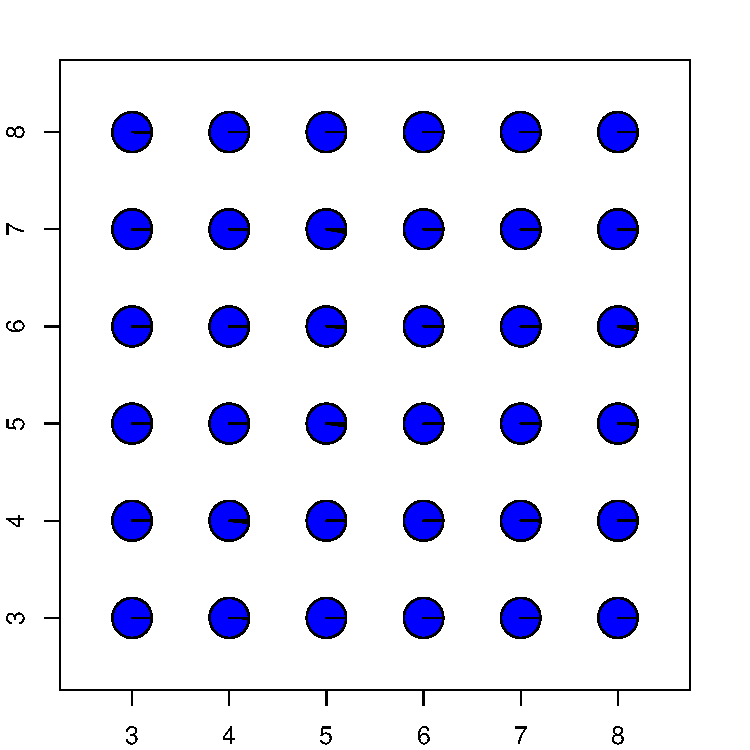
\includegraphics[width=1.8in,height=1.8in]{figs/sims/simK1_sp_pies_K2.pdf}}
		\subcaptionbox{$K=3$\label{simK1_sp_pies:K3}}
			{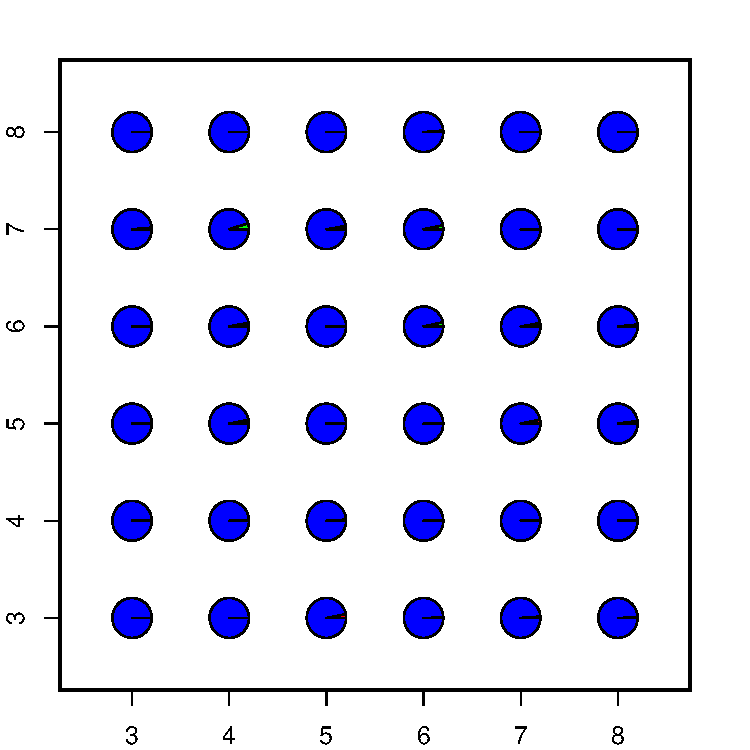
\includegraphics[width=1.8in,height=1.8in]{figs/sims/simK1_sp_pies_K3.pdf}}
		\subcaptionbox{$K=4$\label{simK1_sp_pies:K4}}
			{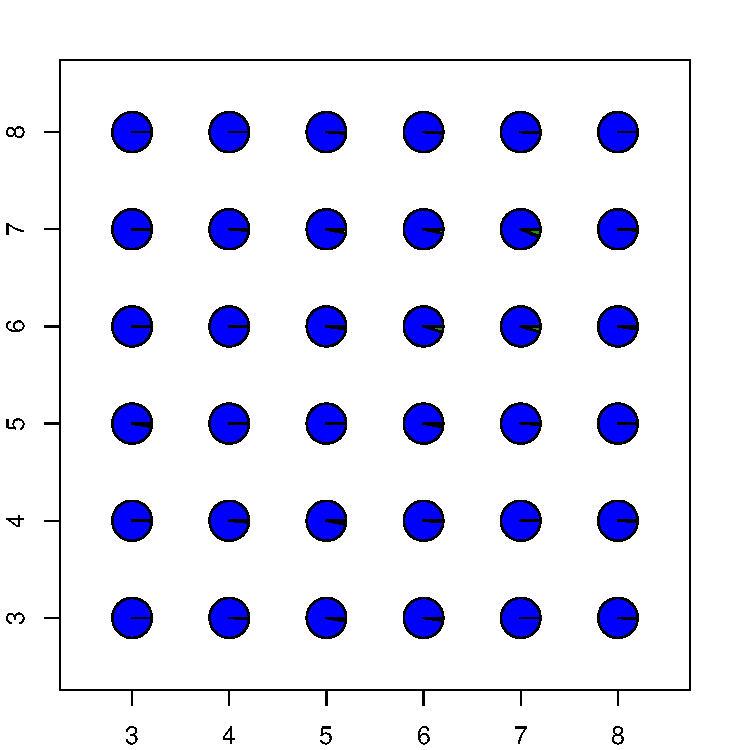
\includegraphics[width=1.8in,height=1.8in]{figs/sims/simK1_sp_pies_K4.pdf}}
		\subcaptionbox{$K=5$\label{simK1_sp_pies:K5}}
			{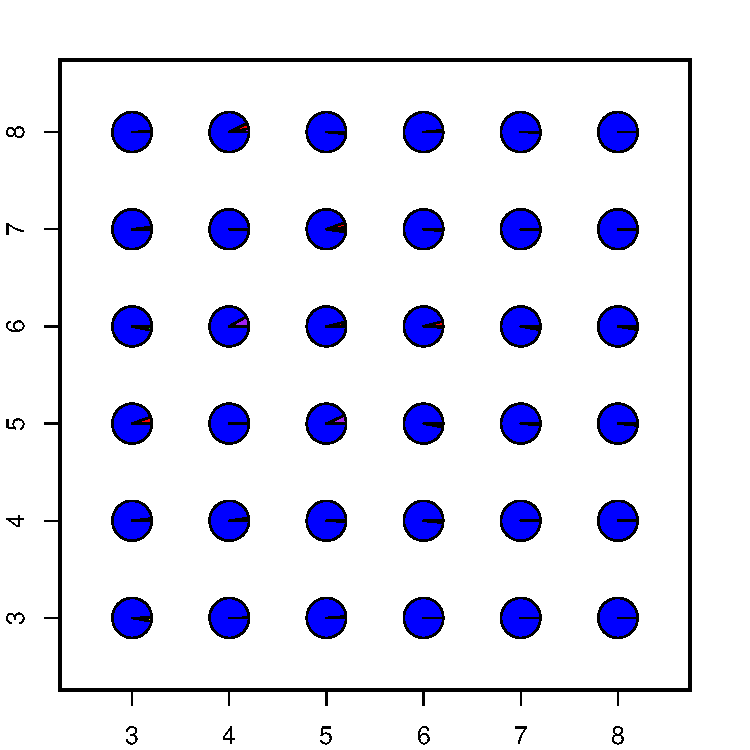
\includegraphics[width=1.8in,height=1.8in]{figs/sims/simK1_sp_pies_K5.pdf}}
		\subcaptionbox{$K=6$\label{simK1_sp_pies:K6}}
			{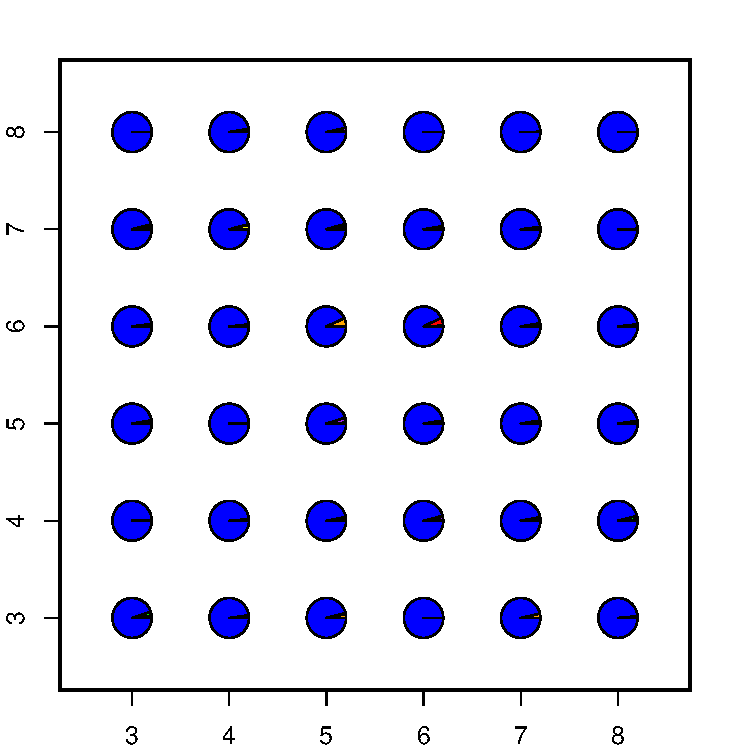
\includegraphics[width=1.8in,height=1.8in]{figs/sims/simK1_sp_pies_K6.pdf}}
		\subcaptionbox{$K=7$\label{simK1_sp_pies:K7}}
			{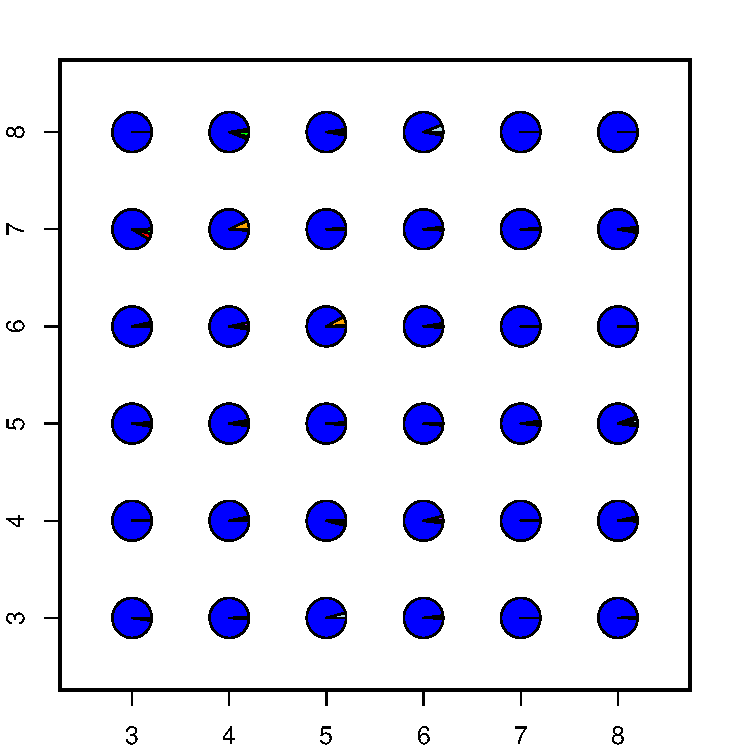
\includegraphics[width=1.8in,height=1.8in]{figs/sims/simK1_sp_pies_K7.pdf}}
	\caption{
	Map of admixture proportions estimated using a spatial model for $K=2$ through 7.
	The data were simulated using 1 cluster with nearest-neighbor symmetric migration between demes.
    }\label{simK1_sp_pies}
\end{figure}

\newpage
\begin{figure}
	\centering
		\subcaptionbox{$K=2$\label{simK2_nsp_pies:K2}}
			{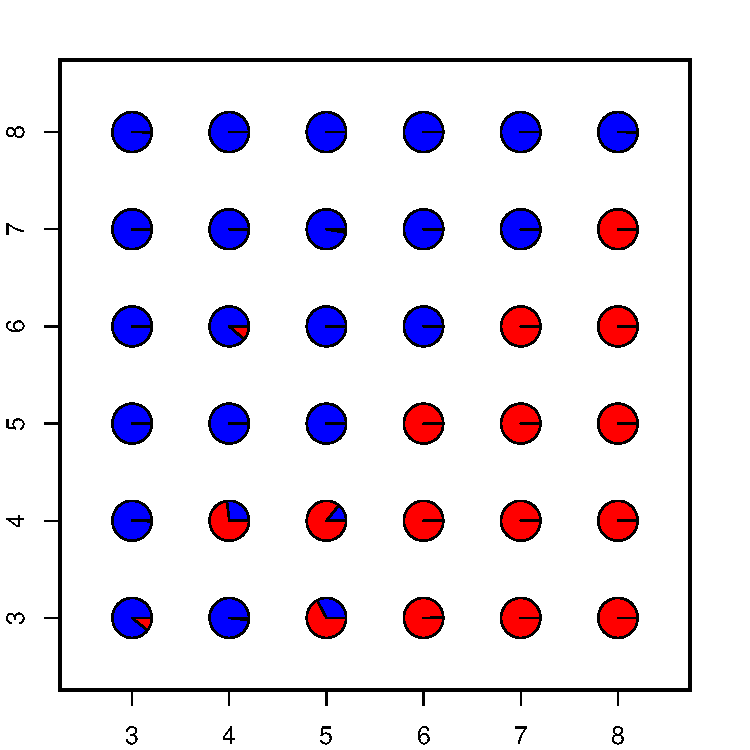
\includegraphics[width=1.8in,height=1.8in]{figs/sims/simK2_nsp_pies_K2.pdf}}
		\subcaptionbox{$K=3$\label{simK2_nsp_pies:K3}}
			{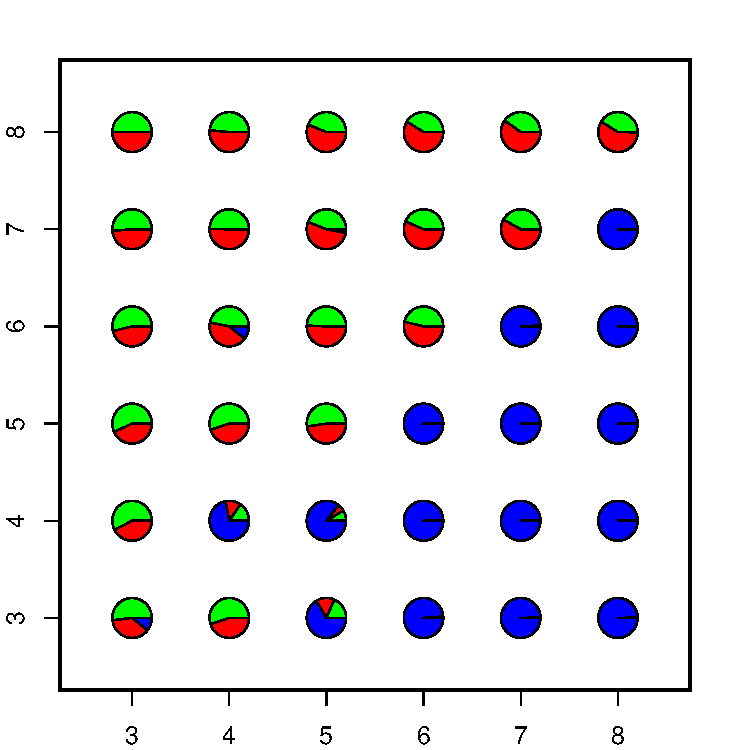
\includegraphics[width=1.8in,height=1.8in]{figs/sims/simK2_nsp_pies_K3.pdf}}
		\subcaptionbox{$K=4$\label{simK2_nsp_pies:K4}}
			{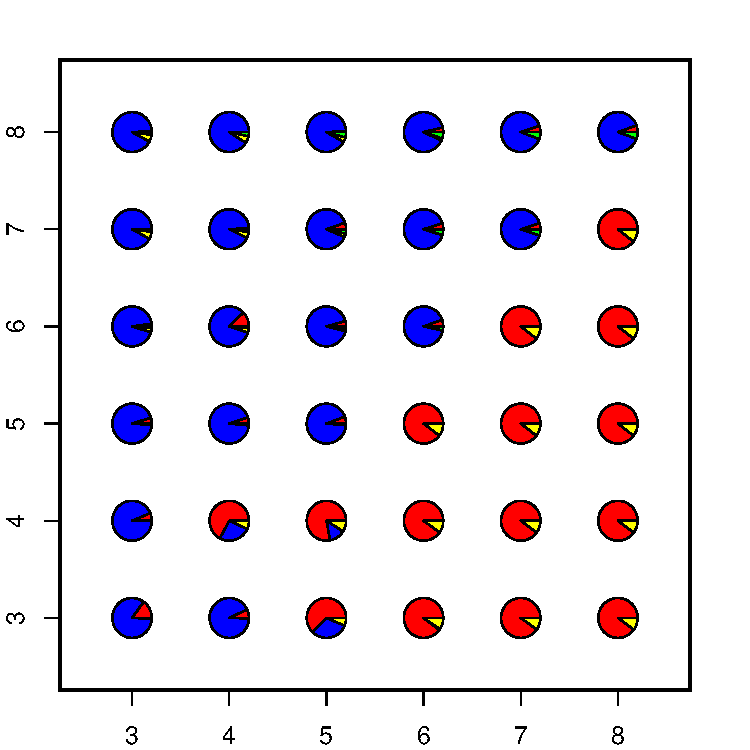
\includegraphics[width=1.8in,height=1.8in]{figs/sims/simK2_nsp_pies_K4.pdf}}
		\subcaptionbox{$K=5$\label{simK2_nsp_pies:K5}}
			{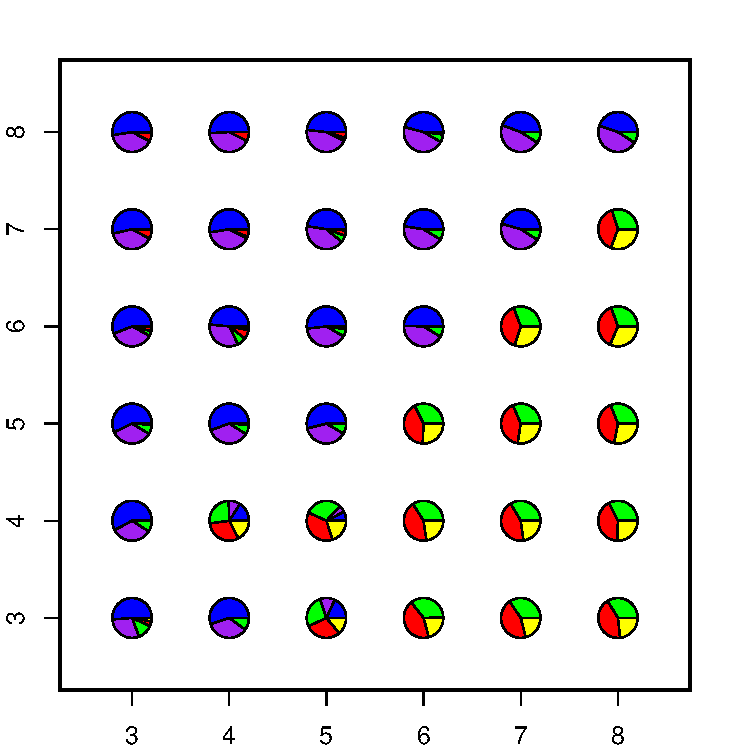
\includegraphics[width=1.8in,height=1.8in]{figs/sims/simK2_nsp_pies_K5.pdf}}
		\subcaptionbox{$K=6$\label{simK2_nsp_pies:K6}}
			{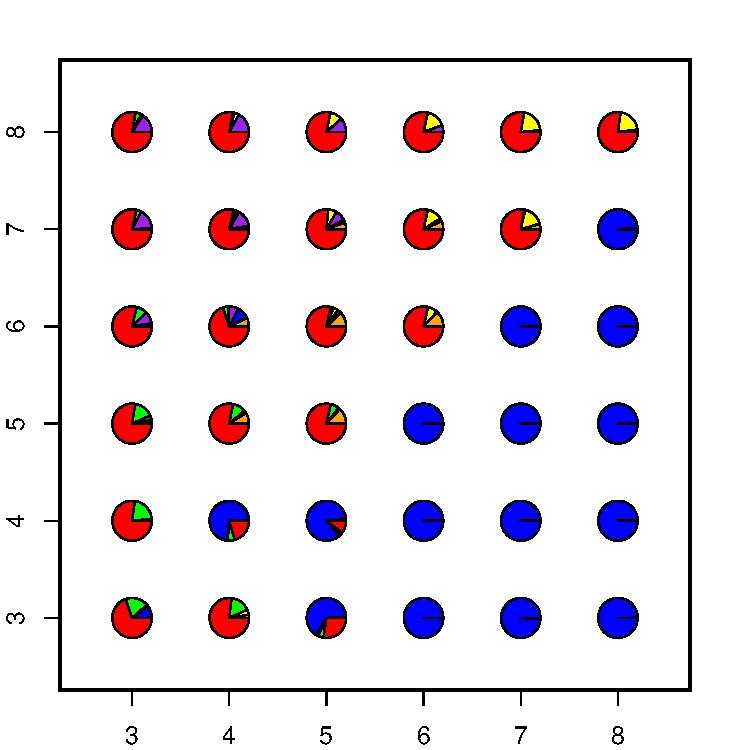
\includegraphics[width=1.8in,height=1.8in]{figs/sims/simK2_nsp_pies_K6.pdf}}
		\subcaptionbox{$K=7$\label{simK2_nsp_pies:K7}}
			{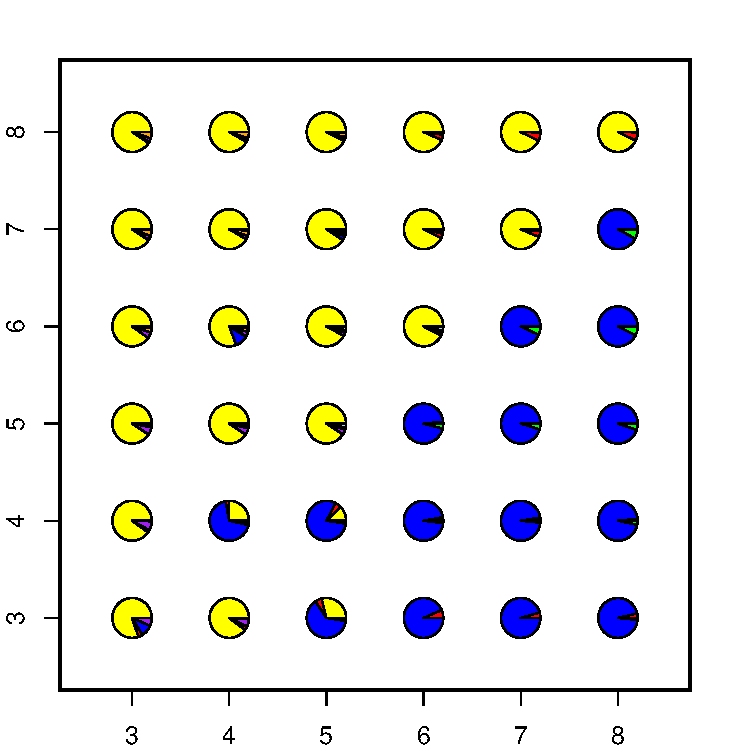
\includegraphics[width=1.8in,height=1.8in]{figs/sims/simK2_nsp_pies_K7.pdf}}
	\caption{
	Map of admixture proportions estimated using a nonspatial model for $K=2$ through 7.
	The data were simulated using two clusters with nearest-neighbor symmetric migration between demes.
    }\label{simK2_nsp_pies}
\end{figure}

\begin{figure}
	\centering
		\subcaptionbox{$K=2$\label{simK2_sp_pies:K2}}
			{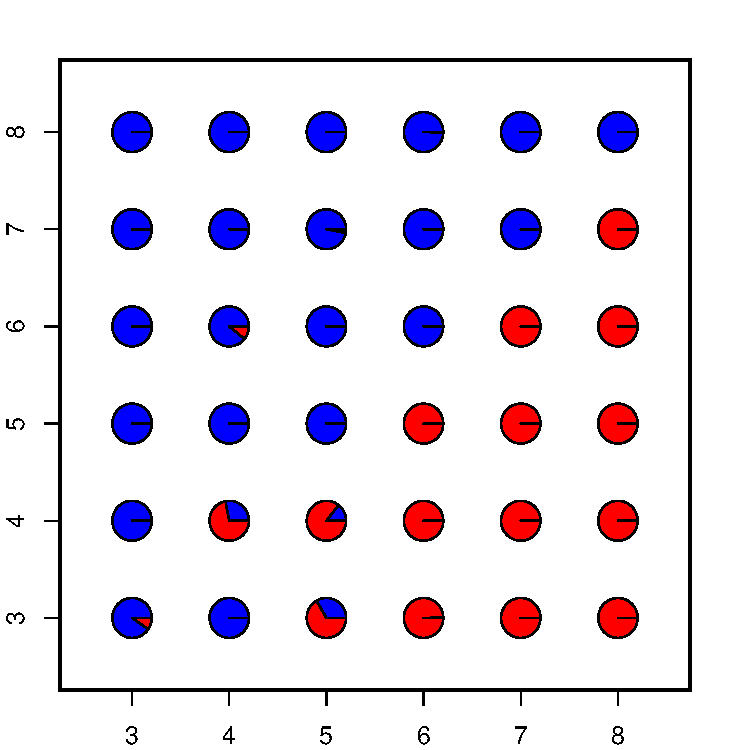
\includegraphics[width=1.8in,height=1.8in]{figs/sims/simK2_sp_pies_K2.pdf}}
		\subcaptionbox{$K=3$\label{simK2_sp_pies:K3}}
			{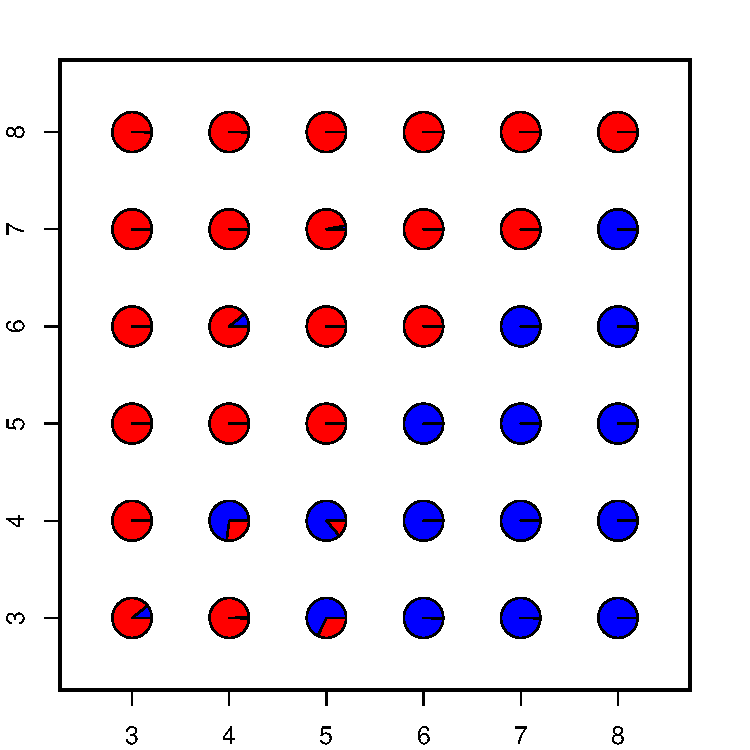
\includegraphics[width=1.8in,height=1.8in]{figs/sims/simK2_sp_pies_K3.pdf}}
		\subcaptionbox{$K=4$\label{simK2_sp_pies:K4}}
			{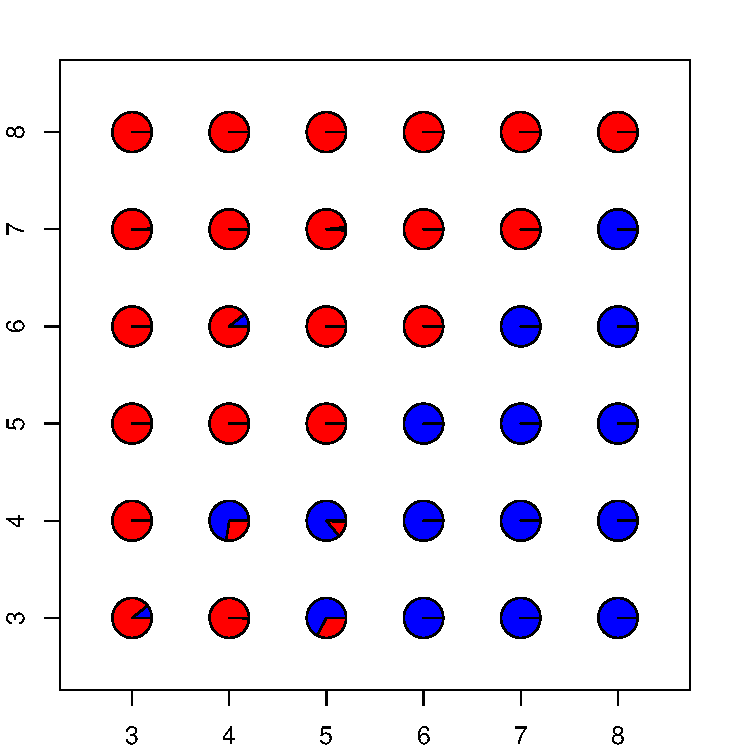
\includegraphics[width=1.8in,height=1.8in]{figs/sims/simK2_sp_pies_K4.pdf}}
		\subcaptionbox{$K=5$\label{simK2_sp_pies:K5}}
			{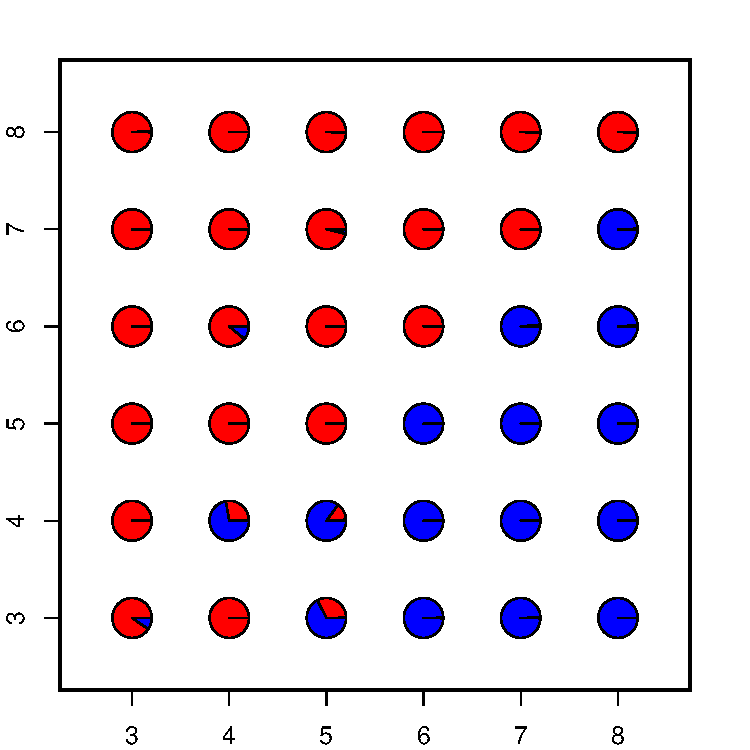
\includegraphics[width=1.8in,height=1.8in]{figs/sims/simK2_sp_pies_K5.pdf}}
		\subcaptionbox{$K=6$\label{simK2_sp_pies:K6}}
			{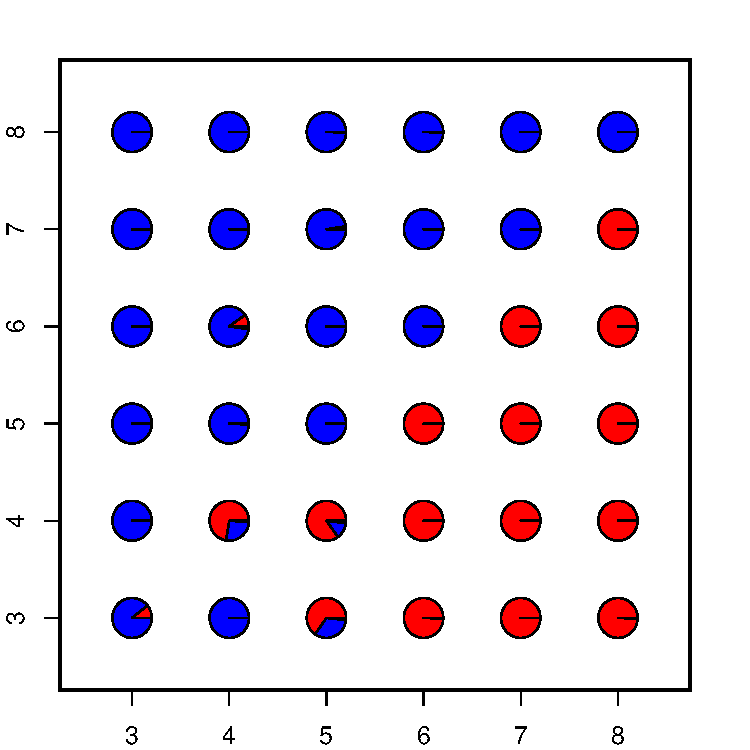
\includegraphics[width=1.8in,height=1.8in]{figs/sims/simK2_sp_pies_K6.pdf}}
		\subcaptionbox{$K=7$\label{simK2_sp_pies:K7}}
			{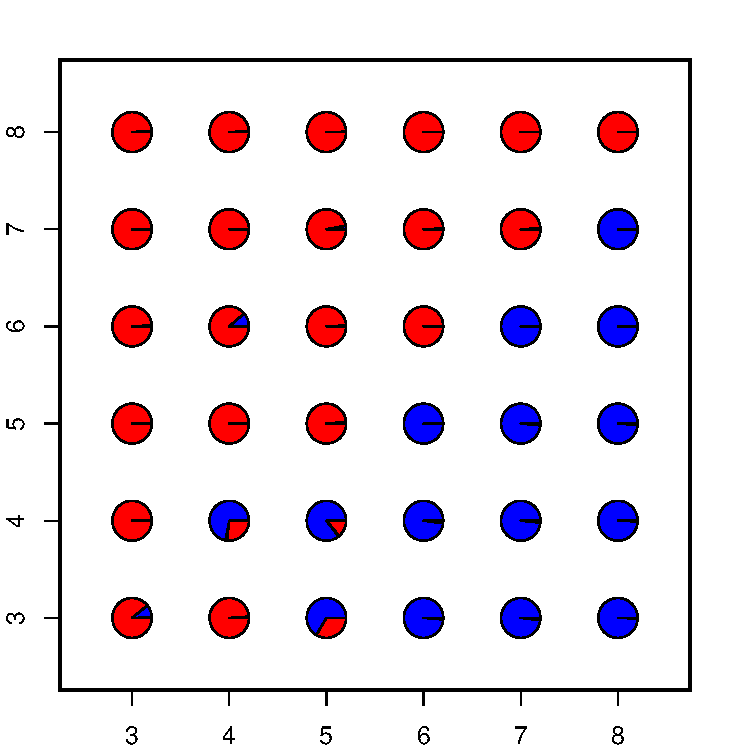
\includegraphics[width=1.8in,height=1.8in]{figs/sims/simK2_sp_pies_K7.pdf}}
	\caption{
	Map of admixture proportions estimated using a spatial model for $K=2$ through 7.
	The data were simulated using two clusters with nearest-neighbor symmetric migration between demes.
    }\label{simK2_sp_pies}
\end{figure}

\begin{figure}
	\centering
		\subcaptionbox{$K=2$\label{simK3_nsp_pies:K2}}
			{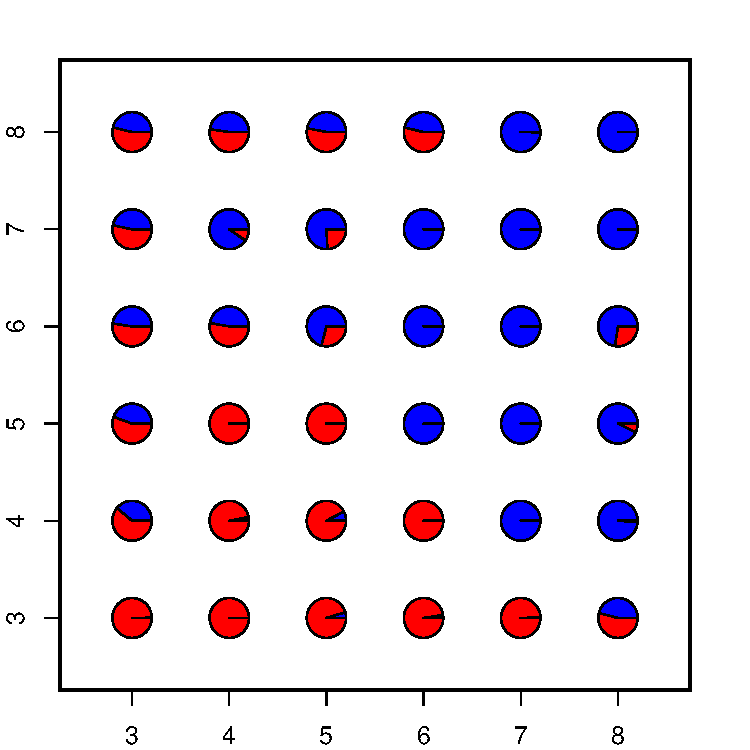
\includegraphics[width=1.8in,height=1.8in]{figs/sims/simK3_nsp_pies_K2.pdf}}
		\subcaptionbox{$K=3$\label{simK3_nsp_pies:K3}}
			{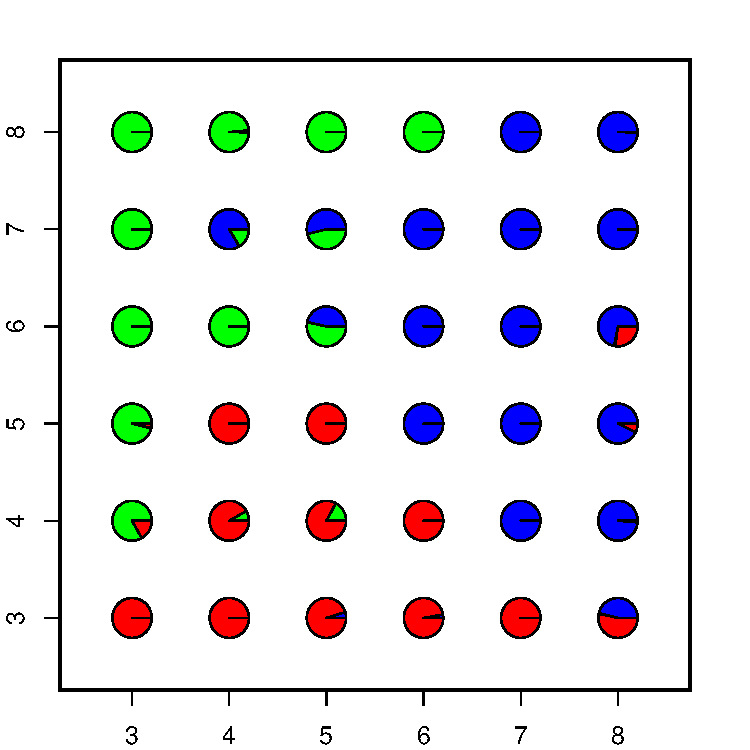
\includegraphics[width=1.8in,height=1.8in]{figs/sims/simK3_nsp_pies_K3.pdf}}
		\subcaptionbox{$K=4$\label{simK3_nsp_pies:K4}}
			{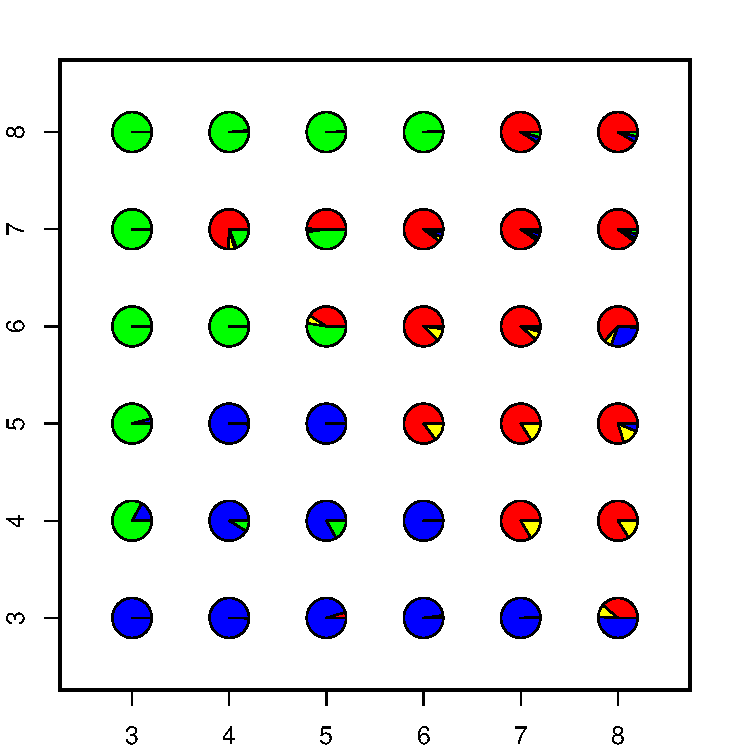
\includegraphics[width=1.8in,height=1.8in]{figs/sims/simK3_nsp_pies_K4.pdf}}
		\subcaptionbox{$K=5$\label{simK3_nsp_pies:K5}}
			{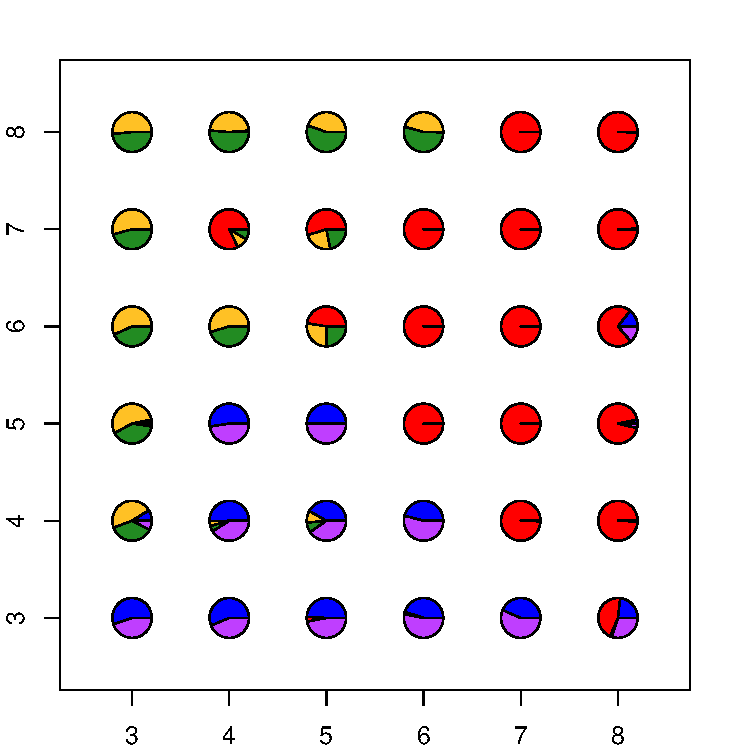
\includegraphics[width=1.8in,height=1.8in]{figs/sims/simK3_nsp_pies_K5.pdf}}
		\subcaptionbox{$K=6$\label{simK3_nsp_pies:K6}}
			{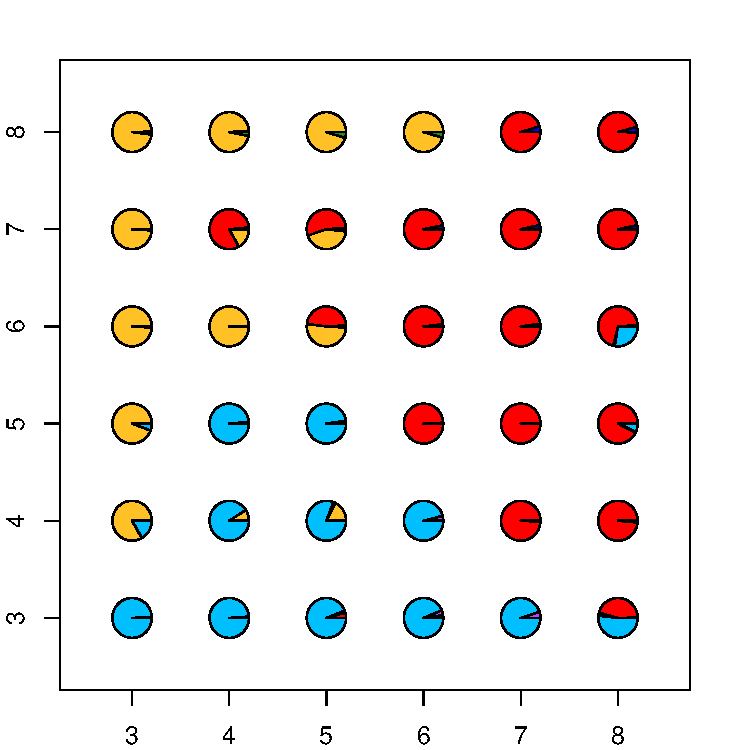
\includegraphics[width=1.8in,height=1.8in]{figs/sims/simK3_nsp_pies_K6.pdf}}
		\subcaptionbox{$K=7$\label{simK3_nsp_pies:K7}}
			{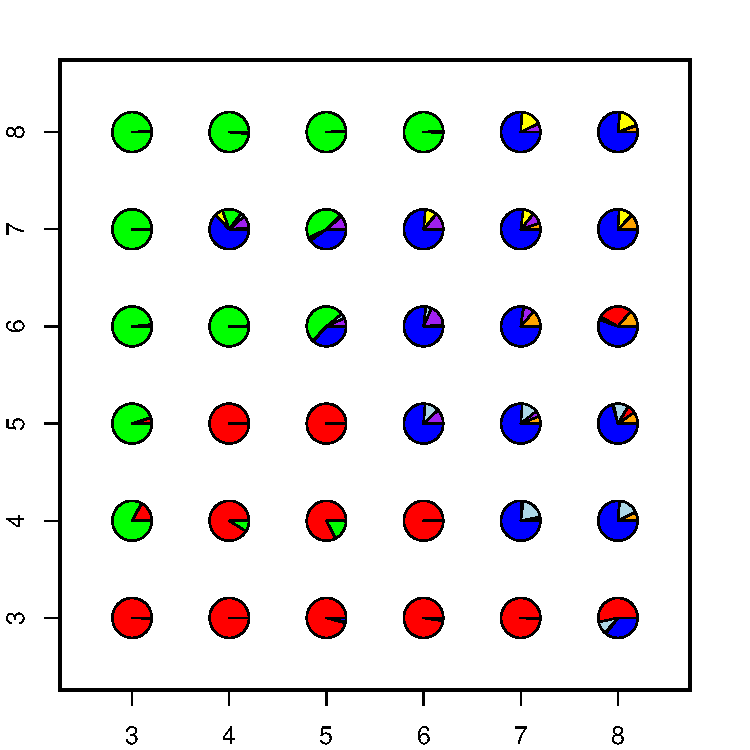
\includegraphics[width=1.8in,height=1.8in]{figs/sims/simK3_nsp_pies_K7.pdf}}
	\caption{
	Map of admixture proportions estimated using a nonspatial model for $K=2$ through 7.
	The data were simulated using three clusters with nearest-neighbor symmetric migration between demes.
    }\label{simK3_nsp_pies}
\end{figure}

\begin{figure}
	\centering
		\subcaptionbox{$K=2$\label{simK3_sp_pies:K2}}
			{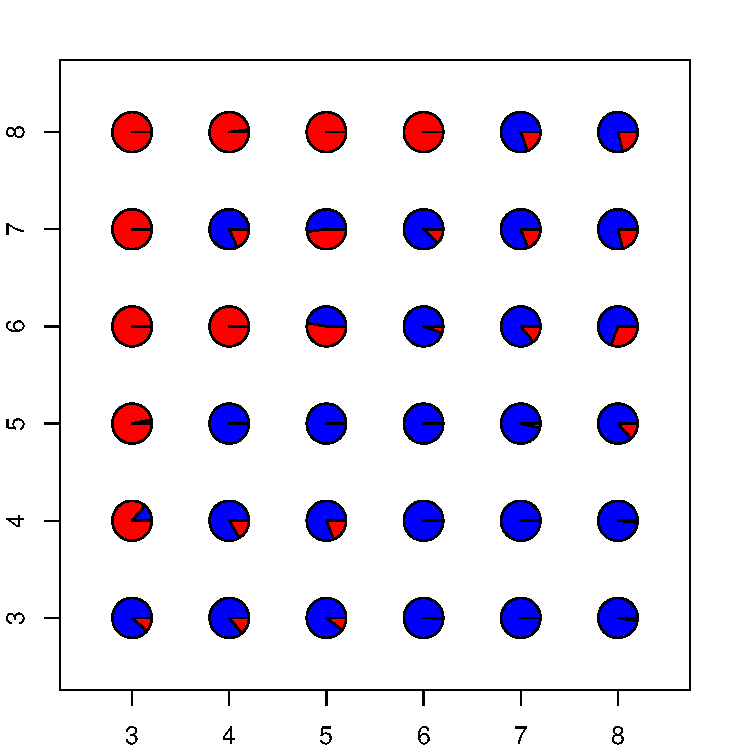
\includegraphics[width=1.8in,height=1.8in]{figs/sims/simK3_sp_pies_K2.pdf}}
		\subcaptionbox{$K=3$\label{simK3_sp_pies:K3}}
			{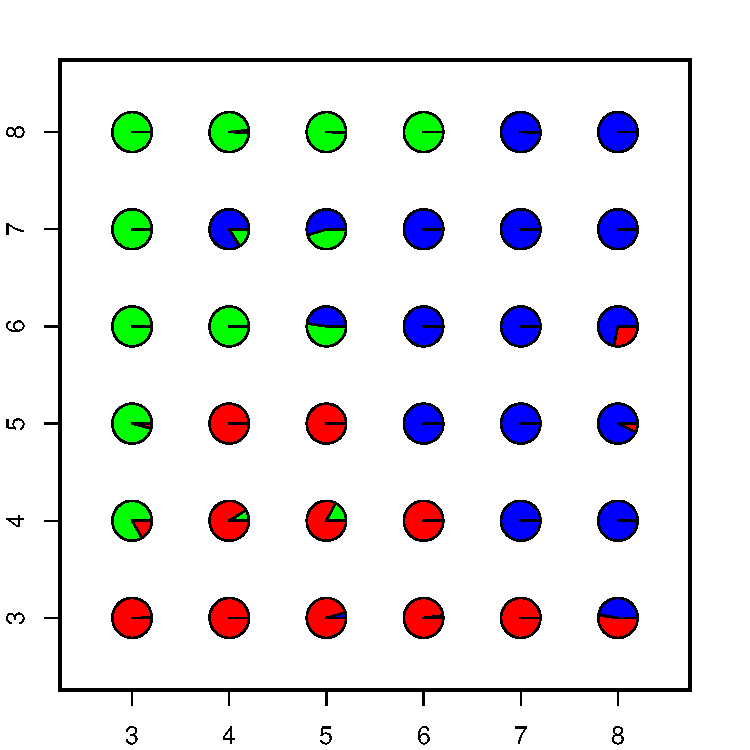
\includegraphics[width=1.8in,height=1.8in]{figs/sims/simK3_sp_pies_K3.pdf}}
		\subcaptionbox{$K=4$\label{simK3_sp_pies:K4}}
			{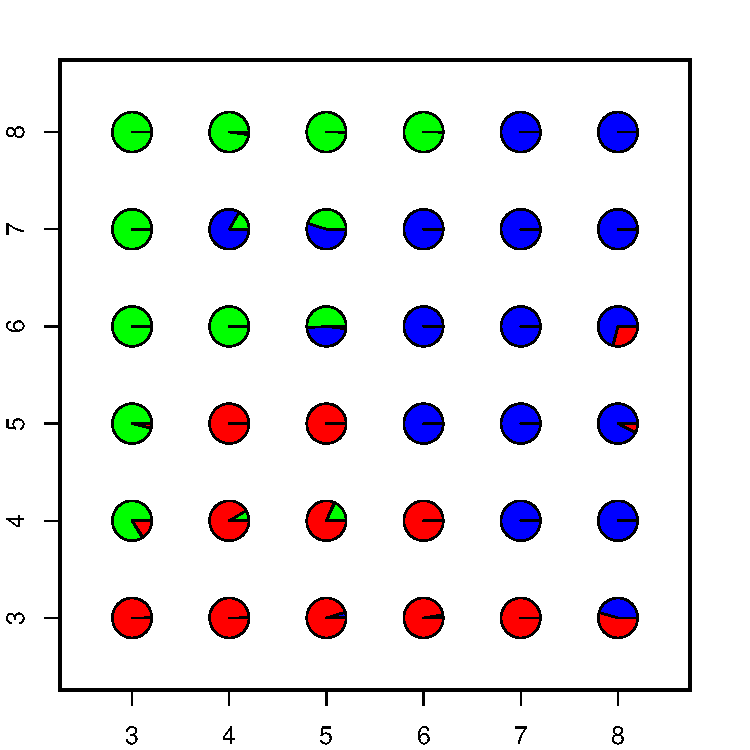
\includegraphics[width=1.8in,height=1.8in]{figs/sims/simK3_sp_pies_K4.pdf}}
		\subcaptionbox{$K=5$\label{simK3_sp_pies:K5}}
			{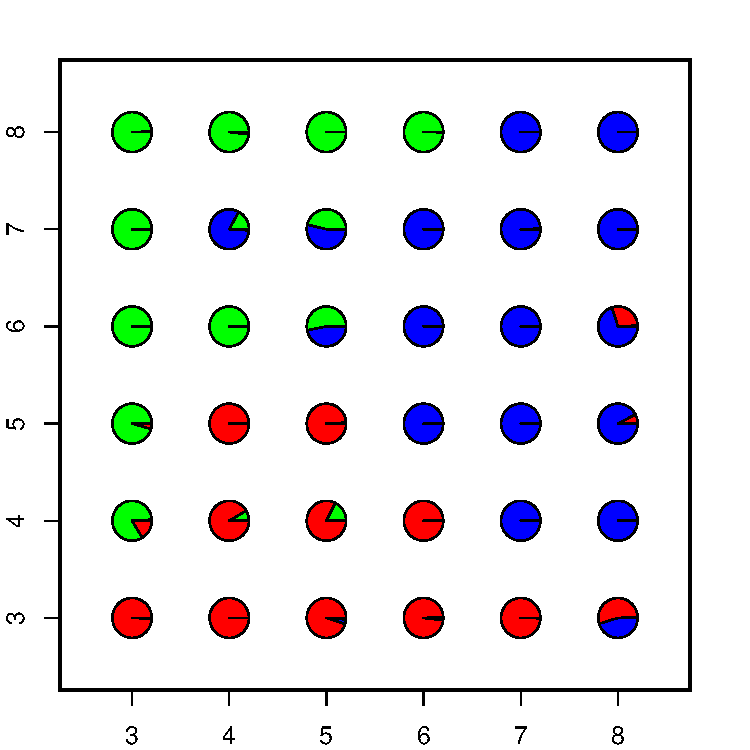
\includegraphics[width=1.8in,height=1.8in]{figs/sims/simK3_sp_pies_K5.pdf}}
		\subcaptionbox{$K=6$\label{simK3_sp_pies:K6}}
			{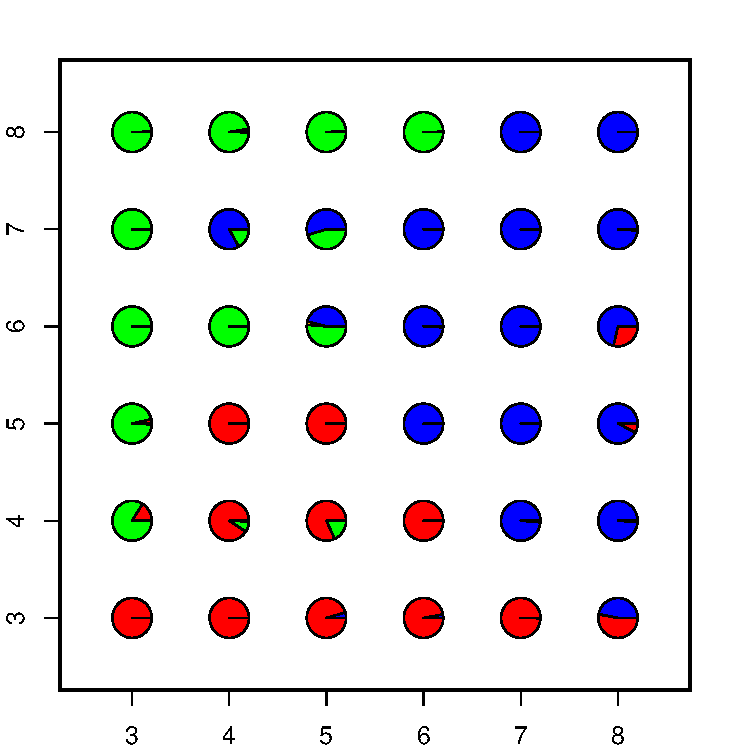
\includegraphics[width=1.8in,height=1.8in]{figs/sims/simK3_sp_pies_K6.pdf}}
		\subcaptionbox{$K=7$\label{simK3_sp_pies:K7}}
			{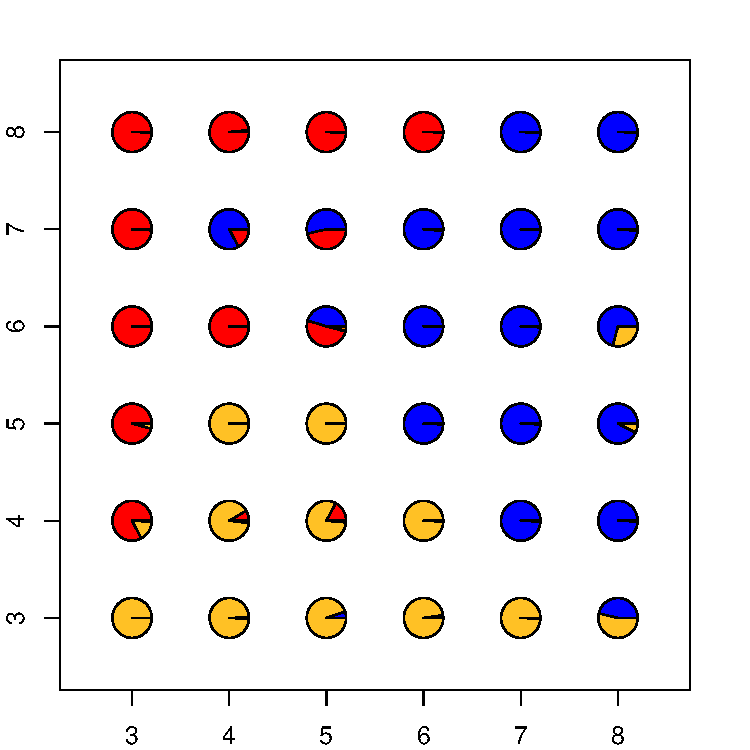
\includegraphics[width=1.8in,height=1.8in]{figs/sims/simK3_sp_pies_K7.pdf}}
	\caption{
	Map of admixture proportions estimated using a spatial model for $K=2$ through 7.
	The data were simulated using three clusters with nearest-neighbor symmetric migration between demes.
    }\label{simK3_sp_pies}
\end{figure}

\newpage
\clearpage
\bibliography{reference.library.tex.bib}

\newpage

\pagenumbering{gobble}

\end{document}
